\documentclass[11pt]{amsart}
\usepackage[margin=1.15in]{geometry}
\usepackage{amsmath,amssymb,amsthm,mathtools}
\usepackage{graphicx,booktabs,multirow}
\usepackage[ruled,vlined,linesnumbered]{algorithm2e}
\usepackage[colorlinks=true,linkcolor=blue!50!black,citecolor=blue!50!black,urlcolor=blue!50!black]{hyperref}
\usepackage[capitalize,nameinlink]{cleveref}
\usepackage{xcolor}

\newtheorem{theorem}{Theorem}[section]
\newtheorem{lemma}[theorem]{Lemma}
\newtheorem{proposition}[theorem]{Proposition}
\newtheorem{corollary}[theorem]{Corollary}
\theoremstyle{definition}
\newtheorem{definition}[theorem]{Definition}
\newtheorem{assumption}[theorem]{Assumption}
\theoremstyle{remark}
\newtheorem{remark}[theorem]{Remark}
\numberwithin{equation}{section}
\crefname{algocf}{Algorithm}{Algorithms}

% ---------- notation ----------
\newcommand{\R}{\mathbb{R}}
\newcommand{\Z}{\mathbb{Z}}
\newcommand{\eps}{\varepsilon}
\newcommand{\nrm}[1]{\lVert #1\rVert}
\newcommand{\ip}[2]{(#1,#2)}
\newcommand{\gradN}{\nabla_{\!N}}
\newcommand{\LapN}{\Delta_N}
\newcommand{\Vh}{\mathcal{V}}
\newcommand{\Vo}{\mathring{\mathcal{V}}}
\newcommand{\Vn}{\mathcal{V}_n}
\newcommand{\LA}{\mathcal{L}_A}
\newcommand{\Bo}{\mathcal{B}}
\newcommand{\Rn}{\mathcal{R}_n}
\newcommand{\Jn}{\mathcal{J}_n}
\newcommand{\Gn}{\mathcal{G}_n}
\newcommand{\Dn}{\mathcal{D}_n}
\newcommand{\Et}{\widetilde{E}}
\newcommand{\nB}[1]{\lVert #1\rVert_{\Bo}}
\newcommand{\nBi}[1]{\lVert #1\rVert_{\Bo^{-1}}}
\newcommand{\Po}{\mathsf{P}_0}
\DeclareMathOperator{\mean}{mean}

\title[Inner iterations for a second-order Cahn--Hilliard scheme]{Solving a second-order energy-stable Cahn--Hilliard scheme by preconditioned descent: global convergence, computable stopping rules, and error estimates}

\author{[Author names withheld for review preparation]}
\address{[Affiliations]}
\email{[e-mail]}

\date{\today}


\renewcommand{\topfraction}{0.9}\renewcommand{\bottomfraction}{0.6}\renewcommand{\textfraction}{0.1}\renewcommand{\floatpagefraction}{0.75}\setcounter{topnumber}{2}\setcounter{totalnumber}{3}
\begin{document}

\begin{abstract}
Second-order, unconditionally energy-stable time discretizations of the Cahn--Hilliard equation are implicit, and in practice their nonlinear step equations are solved only approximately: a few sweeps of a constant-coefficient ``linear iteration'' are performed and the last iterate is accepted. The stability and accuracy statements available for these schemes, however, refer to the exact solution of each step. We study this gap for the modified Crank--Nicolson Fourier pseudo-spectral scheme of Cheng, Wang, Wise and Yue in its practically used form with an $O(\tau^2)$ stabilization $A(\phi^{n+1}-2\phi^n+\phi^{n-1})$. We show that each time step is the minimization of a strongly convex functional and that the linear iteration is exactly a fixed-step preconditioned gradient descent for this functional. This yields convergence of the relaxed iteration from any starting value for every stabilization parameter $A\ge 0$, time step and interface width, provided the relaxation parameter respects a bound determined by the maximum norm on a sublevel set; convergence, without a priori knowledge of the sublevel-set bound, of an Armijo line-search variant and of Newton's method with any positive number of preconditioned conjugate-gradient steps; and an explicit local rate. We then prove a two-sided a posteriori bound relating the residual of any candidate to its distance from the exact step solution, and an exact perturbed energy identity valid for any candidate. These give computable acceptance tests, costing no additional transforms, that guarantee decay of a modified energy for every $\tau>0$ and, with a residual tolerance proportional to $\tau^2$ and under the stated regularity and mesh--time-step conditions, optimal $O(\tau^2+h^m)$ convergence of the \emph{computed} solution in $\ell^\infty(H^{-1})\cap\ell^2(H^1)$; in general the error bound separates the discretization error from the computable algebraic term $(\tau\sum_n\nrm{\Rn(\phi^{n+1})}^2)^{1/2}$. Numerical experiments confirm the theory. The unrelaxed linear iteration can diverge in parameter regimes of practical interest, and relaxation with a fixed number of inner sweeps reduces the observed temporal order, whereas residual-based termination preserves second order. At equal accuracy on a smooth test problem, the computable acceptance rule needs up to $37\%$ fewer transforms than a fixed number of sweeps and $35$--$67\%$ fewer than a tight tolerance. On a droplet merger and an Ostwald-ripening test, the practical rule with an Armijo inner method reproduces the merger and disappearance steps of a tightly converged Newton--PCG solve with $54$--$67\%$ fewer transforms.
\end{abstract}

\subjclass[2020]{65M12, 65M70, 65H10, 65K10, 35K55}
\keywords{Cahn--Hilliard equation, energy stability, Crank--Nicolson, Fourier pseudo-spectral method, inexact solves, preconditioned gradient descent, a posteriori error bound, stopping criteria}

\maketitle

\section{Introduction}\label{sec:intro}

We consider the Cahn--Hilliard equation \cite{CahnHilliard1958} on $\Omega=(0,L)^2$ with periodic boundary conditions,
\begin{equation}\label{eq:ch}
\partial_t\phi=\Delta\mu,\qquad \mu=\phi^3-\phi-\eps^2\Delta\phi,
\end{equation}
the $H^{-1}$ gradient flow of
\begin{equation}\label{eq:energy}
E(\phi)=\int_\Omega\Big(\tfrac14\phi^4-\tfrac12\phi^2\Big)\,dx+\frac{\eps^2}{2}\int_\Omega|\nabla\phi|^2\,dx,\qquad \frac{d}{dt}E(\phi)=-\nrm{\nabla\mu}_{L^2}^2,\qquad \frac{d}{dt}\int_\Omega\phi\,dx=0 .
\end{equation}
Energy-stable time discretizations are standard: convex splitting \cite{Eyre1998}, secant and discrete-gradient methods \cite{DuNicolaides1991,Furihata2001}, second-order convex-splitting schemes \cite{ShenWangWangWise2012,GuanLowengrubWangWise2014,DiegelWangWise2016,ChengWangWiseYue2016}, stabilized linear schemes \cite{FengTangYang2013,LiQiaoTang2016,YanChenWangWise2018,WangYu2018}, and auxiliary-variable formulations \cite{ShenXuYang2018,ShenXuYang2019}.

We study the modified Crank--Nicolson Fourier pseudo-spectral scheme of Cheng, Wang, Wise and Yue \cite{ChengWangWiseYue2016} in its practically used form, with the stabilization $A(\phi^{n+1}-2\phi^n+\phi^{n-1})$ ($\alpha=0$ in \cite{ChengWangWiseYue2016}). Each step is a cubic system, solved in \cite{ChengWangWiseYue2016} by a constant-coefficient \emph{linear iteration}; contraction for $\alpha=0$ is left open there \cite[Remark~2.10]{ChengWangWiseYue2016}. Related $\ell^4$ contraction results are \cite{ZhuGongWang2025,ChenJingLiuWangWang2024}; preconditioned steepest descent and multigrid are used in \cite{FengSalgadoWangWise2017,ChenWangWise2022,GuanLowengrubWangWise2014}. All stability and convergence statements for the scheme concern the \emph{exact} step solution, whereas codes accept an iterate after finitely many sweeps. This paper analyses the scheme \emph{as computed}.

\medskip\noindent\textbf{Main results.} Let $\Rn$ be the step residual, $\Jn$ the step functional, $\Bo$ the constant-coefficient preconditioner and $q=\frac32M^2\theta_N$ with $M$ a maximum-norm bound and $\theta_N\le(A+\sqrt3\eps\tau^{-1/2})^{-1}$ (\cref{sec:scheme}).
\begin{enumerate}
\item $\Jn$ is $1$-strongly convex in $\nBi\cdot$, $\Rn=\nabla\Jn$, and for every candidate $v$
\[
\Et(v,\phi^n)-\Et(\phi^n,\phi^{n-1})+\Dn(v)=\ip{\Rn(v)}{v-\phi^n}\qquad(\text{\cref{prop:convex,thm:identity}}).
\]
\item The linear iteration is $v^{k+1}=v^k-\Bo\Rn(v^k)$. With relaxation $\omega<2/(1+q_0)$ it converges globally for all $A\ge0$, $\tau,\eps>0$; with Armijo backtracking, or Newton--PCG with any positive number of conjugate-gradient steps, without a priori knowledge of $q_0$; locally with factor $\max\{|1-\omega|,|1-\omega(1+q_*)|\}$ (\cref{thm:global,thm:armijo,thm:local,thm:newton}).
\item $\nBi{v-\phi^{n+1}}\le\nB{\Rn(v)}\le(1+q)\nBi{v-\phi^{n+1}}$, with a fully computable $q$ (\cref{cor:effectivity}), and the transform-free tests $|\ip{\Rn(v)}{v-\phi^n}|\le\eta\Dn(v)$, $\nrm{\Rn(v)}\le c_R\tau^2$ give energy decay of the computed sequence for every $\tau>0$ (\cref{thm:apost,thm:energysafe}).
\item With accepted residuals $\rho^n$,
\[
\nrm{e^n}_{-1}+\Big(\tau\sum_{j\le n}\eps^2\nrm{\gradN e^j}^2\Big)^{1/2}\le C\Big(\tau^2+h^m+\Big(\tau\sum_{j<n}\nrm{\rho^j}^2\Big)^{1/2}\Big);
\] hence, under \cref{ass:smooth}, $\tau\le\tau_0$ and $(1+\ln N)^{1/2}(\tau^{3/2}+\tau^{-1/2}h^m)\le c_0'$, $O(\tau^2+h^m)$ under the accuracy test (energy decay needs none of these conditions), and an $O(\tau)$ bound when $\nrm{\rho^n}=O(\tau)$, which a formal expansion identifies as the regime of a fixed number of relaxed sweeps; for the linearisation at $\phi=0$ the growth rate of $K$ relaxed sweeps is proved to carry the first-order error $-\frac{r}{1-r}\lambda^2\tau$, $r=(1-\omega)^K$, nonzero for $\lambda\ne0$, $0<r<1$ (\cref{thm:error,cor:TA,cor:fixedK,prop:fixedK,prop:linfixed}).
\item Experiments (\cref{sec:numerics}) confirm divergence of the unrelaxed iteration, loss of order under fixed relaxed sweeps, sharpness of the a posteriori bound, and agreement of the practical rule (Armijo inner method) with tightly converged Newton--PCG in the reported observables at $54$--$67\%$ fewer transforms on six runs (labyrinthine coarsening, a merger, Ostwald ripening, three droplet patterns).
\end{enumerate}
\medskip\noindent\textbf{Relation to preconditioned-descent theory.} Preconditioned steepest descent for convex-splitting schemes is analysed in \cite{FengSalgadoWangWise2017,ChenWangWise2022}. For the logarithmic (Flory--Huggins) potential and a finite-difference convex-splitting scheme, Diegel, Wang and Wise \cite{DiegelWangWise2025} prove geometric convergence together with positivity of the logarithmic arguments, assuming strict separation of the discrete solution from $\pm1$. Park, Salgado and Wise \cite{ParkSalgadoWise2025} prove linear convergence of preconditioned gradient descent for strongly convex composite functionals when part of the gradient is computed inexactly, with an error term governed by the gradient accuracy. These results concern convergence \emph{within} one implicit step, for other schemes or inexactness models. Here the gradient is exact and the step functional is that of the second-order secant scheme of \cite{ChengWangWiseYue2016}, whose existing linear iteration is the unit-step method. What we add is the treatment of \emph{termination}: a computable two-sided certificate of the algebraic error (\cref{thm:apost,cor:effectivity}), an exact energy identity for arbitrary candidates that turns stopping into a test with guaranteed energy decay of the accepted sequence (\cref{thm:identity,thm:energysafe}), and the propagation of the accepted residuals through the time-stepping error analysis, giving the accumulated term $(\tau\sum\nrm{\rho^j}^2)^{1/2}$ (\cref{thm:error}).

\Cref{sec:scheme} contains the discrete setting and the variational structure, \cref{sec:solver} the inner iterations and termination, \cref{sec:error} the error analysis, \cref{sec:numerics} the experiments and concluding remarks, and the appendix auxiliary proofs and implementation formulas.

\section{Discrete setting and variational structure of a time step}\label{sec:scheme}

\subsection{Grid functions}
Let $N\ge2$ be even, $h=L/N$, $x_{ij}=(ih,jh)$, and $\Vh$ the real $L$-periodic grid functions. For $f,g\in\Vh$,
\[
\ip fg=h^2\!\!\sum_{i,j=0}^{N-1}\!f_{ij}g_{ij},\quad \nrm f=\ip ff^{1/2},\quad \nrm f_\infty=\max_{i,j}|f_{ij}|,\quad f_{ij}=\sum_{k\in K_N}\hat f_ke^{\mathrm i\kappa_k\cdot x_{ij}},
\]
with $K_N=\{k\in\Z^2:-\frac N2<k_1,k_2\le\frac N2\}$, $\kappa_k=2\pi k/L$, $s_k=|\kappa_k|^2$, and $\nrm f^2=L^2\sum_k|\hat f_k|^2$. The collocation Laplacian and the associated forms are
\begin{equation}\label{eq:lapN}
\widehat{(\LapN f)}_k=-s_k\hat f_k,\qquad \langle f,g\rangle_1=\ip{-\LapN f}g,\qquad \nrm{\gradN f}^2=L^2\sum_ks_k|\hat f_k|^2 .
\end{equation}
Let $\mean(f)=|\Omega|^{-1}\ip f1=\hat f_0$, $\Vo=\{f:\mean(f)=0\}$, $\Po f=f-\mean(f)$, and on $\Vo$
\begin{equation}\label{eq:hm1}
\nrm f_{-1}^2=\ip{(-\LapN)^{-1}f}f=L^2\sum_{k\ne0}s_k^{-1}|\hat f_k|^2 .
\end{equation}
Products such as $\phi^3$ are evaluated pointwise.

\begin{lemma}\label{lem:discrete}
For $f\in\Vo$: {\rm(a)} $\nrm f^2\le\nrm f_{-1}\nrm{\gradN f}$; {\rm(b)} $\nrm f\le\frac L{2\pi}\nrm{\gradN f}$; {\rm(c)} $\nrm f_\infty\le C_N\nrm{\gradN f}$, $C_N=\frac{\sqrt2}{\pi}(1+\ln N)^{1/2}$.
\end{lemma}

\begin{proof}
(a) $\nrm f^2=L^2\sum_{k\ne0}(s_k^{-1/2}|\hat f_k|)(s_k^{1/2}|\hat f_k|)\le(L^2\sum s_k^{-1}|\hat f_k|^2)^{1/2}(L^2\sum s_k|\hat f_k|^2)^{1/2}$. (b) $s_k\ge(2\pi/L)^2$ for $k\ne0$. (c) \Cref{app:sobolev}.
\end{proof}

\subsection{The scheme}
Let $\tau>0$, $A\ge0$ and
\begin{equation}\label{eq:chi}
\chi(a,b)=\tfrac14(a^2+b^2)(a+b),\qquad \chi(a,b)(a-b)=\tfrac14(a^4-b^4).
\end{equation}
Given $\phi^n,\phi^{n-1}$ with $\mean(\phi^n)=\mean(\phi^{n-1})$ and $\phi^{-1}:=\phi^0$, the scheme \cite{ChengWangWiseYue2016} ($\alpha=0$) is
\begin{subequations}\label{eq:scheme}
\begin{align}
\tau^{-1}(\phi^{n+1}-\phi^n)&=\LapN\mu^{n+1/2},\\
\mu^{n+1/2}&=\chi(\phi^{n+1},\phi^n)-\big(\tfrac32\phi^n-\tfrac12\phi^{n-1}\big)-\eps^2\LapN\big(\tfrac34\phi^{n+1}+\tfrac14\phi^{n-1}\big)\notag\\
&\qquad+A\big(\phi^{n+1}-2\phi^n+\phi^{n-1}\big).
\end{align}
\end{subequations}
Since $\widehat{(\LapN g)}_0=0$, $\mean(\phi^{n+1})=\mean(\phi^n)$. The discrete and modified energies are
\begin{equation}\label{eq:modE}
E_N(\phi)=\big(\tfrac14\phi^4-\tfrac12\phi^2,1\big)+\tfrac{\eps^2}{2}\nrm{\gradN\phi}^2,\qquad
\Et(a,b)=E_N(a)+\big(\tfrac14+\tfrac A2\big)\nrm{a-b}^2+\tfrac{\eps^2}{8}\nrm{\gradN(a-b)}^2 .
\end{equation}

\subsection{The preconditioner and its metric}
Let $\LA=\tau^{-1}-A\LapN+\frac34\eps^2\LapN^2$ and $\Bo=\LA^{-1}(-\LapN)$ on $\Vo$, with symbols
\begin{equation}\label{eq:symbols}
\lambda_k=\tau^{-1}+As_k+\tfrac34\eps^2s_k^2,\qquad \beta_k=s_k/\lambda_k\quad(k\ne0).
\end{equation}
Then $\Bo$ is symmetric positive definite on $\Vo$ and, for $f,g\in\Vo$,
\begin{equation}\label{eq:Bnorm}
\nBi f^2=L^2\sum_{k\ne0}\beta_k^{-1}|\hat f_k|^2=\tfrac1\tau\nrm f_{-1}^2+A\nrm f^2+\tfrac34\eps^2\nrm{\gradN f}^2,\qquad \nB g^2=L^2\sum_{k\ne0}\beta_k|\hat g_k|^2,
\end{equation}
\begin{equation}\label{eq:duality}
\ip gf\le\nB g\nBi f,\qquad \nB g=\sup_{0\ne f\in\Vo}\frac{\ip gf}{\nBi f}.
\end{equation}
By the arithmetic--geometric mean inequality $\tau^{-1}+\frac34\eps^2s^2\ge2(\frac34\eps^2\tau^{-1})^{1/2}s=\sqrt3\,\eps\tau^{-1/2}s$, with equality at $s^2=\frac4{3\eps^2\tau}$. Hence
\begin{equation}\label{eq:theta}
\theta_N:=\max_{k\ne0}\beta_k\le\sup_{s>0}\frac{s}{\tau^{-1}+As+\frac34\eps^2s^2}=\frac{1}{A+\sqrt3\,\eps\,\tau^{-1/2}},
\end{equation}
\begin{equation}\label{eq:normequiv}
\nrm f^2\le\theta_N\nBi f^2,\qquad \tfrac34\eps^2\nrm{\gradN f}^2\le\nBi f^2,\qquad \tfrac1\tau\nrm f_{-1}^2\le\nBi f^2\qquad(f\in\Vo).
\end{equation}
The bound \eqref{eq:theta} is uniform in $N$.

\subsection{Residual, step functional and convexity}\label{sec:variational}
Fix $n$, let $\Vn=\{v\in\Vh:\mean(v)=\mean(\phi^n)\}$, $\tilde\phi^n=\frac32\phi^n-\frac12\phi^{n-1}$, $\ell_n=\tilde\phi^n+A(2\phi^n-\phi^{n-1})$, and for $v\in\Vn$
\begin{align}
\mu_n(v)&=\chi(v,\phi^n)-\tilde\phi^n-\eps^2\LapN\big(\tfrac34v+\tfrac14\phi^{n-1}\big)+A\big(v-2\phi^n+\phi^{n-1}\big),\notag\\
\Rn(v)&=\tau^{-1}(-\LapN)^{-1}(v-\phi^n)+\Po\mu_n(v)\in\Vo .\label{eq:residual}
\end{align}
Applying $-\LapN$ (injective on $\Vo$),
\begin{equation}\label{eq:perturbed-scheme}
\tau^{-1}(v-\phi^n)=\LapN\mu_n(v)-\LapN\Rn(v),
\end{equation}
so $v$ solves \eqref{eq:scheme} iff $\Rn(v)=0$. With
\begin{equation}\label{eq:G}
G(a,b)=\int_0^a\chi(s,b)\,ds=\tfrac{a^4}{16}+\tfrac{a^3b}{12}+\tfrac{a^2b^2}{8}+\tfrac{ab^3}{4},\quad \chi_a=\partial_a\chi=\tfrac14(3a^2+2ab+b^2)=\tfrac14\big(2a^2+(a+b)^2\big),
\end{equation}
define on $\Vn$
\begin{equation}\label{eq:J}
\Jn(v)=\tfrac1{2\tau}\nrm{v-\phi^n}_{-1}^2+\big(G(v,\phi^n),1\big)+\tfrac38\eps^2\nrm{\gradN v}^2+\tfrac{\eps^2}{4}\langle\phi^{n-1},v\rangle_1+\tfrac A2\nrm v^2-\ip{\ell_n}{v}.
\end{equation}

\begin{proposition}\label{prop:convex}
Let $v,w\in\Vn$, $d\in\Vo$ and $j(t)=\Jn(v+td)$.
\begin{enumerate}
\item[(i)] $j'(0)=\ip{\Rn(v)}d$ and $j''(t)=\nBi d^2+\ip{\chi_a(v+td,\phi^n)d}{d}\ge\nBi d^2$.
\item[(ii)] $\Jn(w)=\Jn(v)+\ip{\Rn(v)}{w-v}+\int_0^1(1-t)\,j_{w-v}''(t)\,dt\ge\Jn(v)+\ip{\Rn(v)}{w-v}+\frac12\nBi{w-v}^2$, where $j_{w-v}(t)=\Jn(v+t(w-v))$.
\item[(iii)] $\Jn$ has a unique minimizer on $\Vn$; it is the unique solution $\phi^{n+1}$ of \eqref{eq:scheme}.
\item[(iv)] With $\Jn^*=\Jn(\phi^{n+1})$,
\begin{equation}\label{eq:PL}
\tfrac12\nBi{v-\phi^{n+1}}^2\le\Jn(v)-\Jn^*\le\tfrac12\nB{\Rn(v)}^2,\qquad \nBi{v-\phi^{n+1}}\le\nB{\Rn(v)} .
\end{equation}
\end{enumerate}
\end{proposition}

\begin{proof}
(i) Term by term, using $\partial_a G=\chi$, $\ip{(-\LapN)^{-1}(v-\phi^n)}{d}$ for the first term and the symmetry of $\langle\cdot,\cdot\rangle_1$,
\begin{align*}
j'(0)&=\Big(\tfrac1\tau(-\LapN)^{-1}(v-\phi^n)+\chi(v,\phi^n)-\tfrac34\eps^2\LapN v-\tfrac14\eps^2\LapN\phi^{n-1}+Av-\ell_n,\ d\Big)\\
&=\Big(\tfrac1\tau(-\LapN)^{-1}(v-\phi^n)+\mu_n(v),d\Big),
\end{align*}
since $-\ell_n+Av=-\tilde\phi^n+A(v-2\phi^n+\phi^{n-1})$; as $\mean(d)=0$, $\mu_n$ may be replaced by $\Po\mu_n$. Differentiating again, $j''(t)=\frac1\tau\nrm d_{-1}^2+\frac34\eps^2\nrm{\gradN d}^2+A\nrm d^2+\ip{\chi_a(v+td,\phi^n)d}{d}$, and $\chi_a\ge0$ by \eqref{eq:G}.
(ii) Taylor's formula $j(1)=j(0)+j'(0)+\int_0^1(1-t)j''(t)\,dt$ and (i).
(iii) By \cref{lem:Jlower}, $\Jn(v)\to\infty$ as $\nrm{\gradN v}\to\infty$ in the finite-dimensional affine space $\Vn$; by (ii) $\Jn$ is strictly convex. The minimizer is the unique critical point, $\Rn=0$, i.e.\ \eqref{eq:scheme}.
(iv) (ii) with $(v,w)\to(\phi^{n+1},v)$ gives the left inequality. (ii) with $w=\phi^{n+1}$, \eqref{eq:duality} and $xy\le\frac12x^2+\frac12y^2$ give $\Jn^*\ge\Jn(v)-\nB{\Rn(v)}\nBi{\phi^{n+1}-v}+\frac12\nBi{\phi^{n+1}-v}^2\ge\Jn(v)-\frac12\nB{\Rn(v)}^2$. Combining both, $\nBi{v-\phi^{n+1}}\le\nB{\Rn(v)}$.
\end{proof}

\begin{lemma}\label{lem:Jlower}
For $a,b,\ell\in\R$,
\begin{equation}\label{eq:quartic}
G(a,b)-\tfrac{a^4}{32}+\tfrac{b^4}{4}=\Big(\tfrac{a^2}{4\sqrt2}+\tfrac{\sqrt2\,ab}{6}\Big)^2+b^2\Big(\tfrac5{72}a^2+\tfrac14ab+\tfrac14b^2\Big)\ge0,\qquad \tfrac{a^4}{32}-\ell a\ge-\tfrac32|\ell|^{4/3}.
\end{equation}
Consequently, with $C_{J,n}=\big(\frac14(\phi^n)^4+\frac32|\ell_n|^{4/3},1\big)+\frac{\eps^2}{8}\nrm{\gradN\phi^{n-1}}^2$,
\begin{equation}\label{eq:sublevel-linf}
\Jn(v)\ge\tfrac{\eps^2}{4}\nrm{\gradN v}^2-C_{J,n},\qquad \Jn(v)\le\bar J\ \Rightarrow\ \nrm v_\infty\le|\mean(\phi^n)|+\tfrac{2C_N}{\eps}\big(\bar J+C_{J,n}\big)^{1/2}.
\end{equation}
\end{lemma}

\begin{proof}
Expanding the square, $(\frac{a^2}{4\sqrt2}+\frac{\sqrt2ab}{6})^2=\frac{a^4}{32}+\frac{a^3b}{12}+\frac{a^2b^2}{18}$, and $\frac18-\frac1{18}=\frac5{72}$, which proves the identity in \eqref{eq:quartic}; the quadratic form $\frac5{72}x^2+\frac14x+\frac14$ has discriminant $\frac1{16}-\frac5{72}=-\frac1{144}<0$. The scalar function $a\mapsto\frac{a^4}{32}-\ell a$ is minimal at $a^3=8\ell$, with value $\frac12|\ell|^{4/3}-2|\ell|^{4/3}$. In \eqref{eq:J}, $\frac{\eps^2}4\langle\phi^{n-1},v\rangle_1\ge-\frac{\eps^2}8(\nrm{\gradN v}^2+\nrm{\gradN\phi^{n-1}}^2)$, the remaining terms are nonnegative, and $\frac38-\frac18=\frac14$. For the last claim apply \cref{lem:discrete}(c) to $v-\mean(v)$.
\end{proof}

\subsection{Secant calculus and a spectral bound}
For $a,b,c\in\R$,
\begin{equation}\label{eq:secantD}
\begin{gathered}
\chi(a,b)-\chi(c,b)=D(a,c;b)(a-c),\\
D(a,c;b)=\tfrac14\big(a^2+ac+c^2+b(a+c)+b^2\big)=\tfrac18\big[(a+c)^2+(a+b)^2+(b+c)^2\big],
\end{gathered}
\end{equation}
which follows from $a^3-c^3=(a-c)(a^2+ac+c^2)$ and $a^2-c^2=(a-c)(a+c)$. If $|a|,|b|,|c|\le M$, then
\begin{equation}\label{eq:Dbound}
0\le D(a,c;b)\le\tfrac18\cdot3\cdot(2M)^2=\tfrac32M^2,\qquad 0\le\chi_a(a,b)=D(a,a;b)\le\tfrac32M^2 .
\end{equation}
Set
\begin{equation}\label{eq:q}
q(M)=\tfrac32M^2\theta_N .
\end{equation}

\begin{lemma}\label{lem:spectral}
Let $0\le D\in\Vh$ with $\nrm D_\infty\le\frac32M^2$ and $T=\Bo\Po D:\Vo\to\Vo$. Then $T$ is self-adjoint and positive semi-definite in $\ip{\Bo^{-1}\cdot}{\cdot}$, its spectrum lies in $[0,q(M)]$, and for every polynomial $p$
\[
\nBi{p(T)u}\le\max_{\lambda\in[0,q(M)]}|p(\lambda)|\,\nBi u\qquad(u\in\Vo).
\]
\end{lemma}

\begin{proof}
For $u,w\in\Vo$, $\ip{\Bo^{-1}Tu}{w}=\ip{\Po Du}{w}=\ip{Du}{w}$, which is symmetric, and $0\le\ip{Du}u\le\frac32M^2\nrm u^2\le q(M)\nBi u^2$ by \eqref{eq:normequiv}. The spectral theorem in $(\Vo,\ip{\Bo^{-1}\cdot}\cdot)$ gives the rest.
\end{proof}

For $w\in\Vn$ and $d\in\Vo$ with $\nrm w_\infty,\nrm{\phi^n}_\infty\le M$, \cref{prop:convex}(i), \eqref{eq:Dbound} and \cref{lem:spectral} give
\begin{equation}\label{eq:hessbound}
\nBi d^2\le\frac{d^2}{dt^2}\Jn(w+td)\Big|_{t=0}\le\big(1+q(M)\big)\nBi d^2 .
\end{equation}

\subsection{An energy identity for arbitrary candidates}
\begin{theorem}\label{thm:identity}
For $v\in\Vn$ let $\delta=v-\phi^n$, $\delta_0=\phi^n-\phi^{n-1}$, $\delta_2=\delta-\delta_0$ and
\begin{equation}\label{eq:dissipation}
\Dn(v)=\tfrac1\tau\nrm\delta_{-1}^2+\big(\tfrac14+\tfrac A2\big)\nrm{\delta_2}^2+\tfrac{\eps^2}8\nrm{\gradN\delta_2}^2\ge0 .
\end{equation}
Then
\begin{equation}\label{eq:identity}
\Et(v,\phi^n)-\Et(\phi^n,\phi^{n-1})+\Dn(v)=\ip{\Rn(v)}{v-\phi^n}.
\end{equation}
\end{theorem}

\begin{proof}
Write $a=v$, $b=\phi^n$, $c=\phi^{n-1}$, so $\delta=a-b$, $\delta_0=b-c$, $\delta_2=a-2b+c$. By \eqref{eq:residual} and $\mean(\delta)=0$, $\ip{\Rn(v)}\delta=\frac1\tau\nrm\delta_{-1}^2+\ip{\mu_n(v)}\delta$. With the polarization identities
\[
\ip{x-y}{x}=\tfrac12\big(\nrm x^2-\nrm y^2+\nrm{x-y}^2\big),\qquad \ip{x+y}{x-y}=\nrm x^2-\nrm y^2,
\]
and their analogues for $\langle\cdot,\cdot\rangle_1$, the four parts of $\mu_n(v)$ give
\begin{align*}
\ip{\chi(a,b)}{a-b}&=\big(\tfrac14a^4-\tfrac14b^4,1\big),\\
-\ip{\tfrac32b-\tfrac12c}{a-b}&=-\tfrac12\ip{a+b}{a-b}+\tfrac12\ip{\delta_2}{\delta}\\
&=-\tfrac12\big(\nrm a^2-\nrm b^2\big)+\tfrac14\big(\nrm\delta^2-\nrm{\delta_0}^2+\nrm{\delta_2}^2\big),\\
\eps^2\big\langle\tfrac34a+\tfrac14c,a-b\big\rangle_1&=\eps^2\big\langle\tfrac12(a+b)+\tfrac14\delta_2,a-b\big\rangle_1\\
&=\tfrac{\eps^2}2\big(\nrm{\gradN a}^2-\nrm{\gradN b}^2\big)+\tfrac{\eps^2}8\big(\nrm{\gradN\delta}^2-\nrm{\gradN\delta_0}^2+\nrm{\gradN\delta_2}^2\big),\\
A\ip{\delta_2}{\delta}&=\tfrac A2\big(\nrm\delta^2-\nrm{\delta_0}^2+\nrm{\delta_2}^2\big),
\end{align*}
where $\delta_2=\delta-\delta_0$ was used in the form $\ip{\delta_2}{\delta}=\frac12(\nrm\delta^2-\nrm{\delta_0}^2+\nrm{\delta_2}^2)$, and $\frac34a+\frac14c=\frac12(a+b)+\frac14(a-2b+c)$. Summing, $\ip{\mu_n(v)}\delta=E_N(a)-E_N(b)+(\frac14+\frac A2)(\nrm\delta^2-\nrm{\delta_0}^2)+\frac{\eps^2}8(\nrm{\gradN\delta}^2-\nrm{\gradN\delta_0}^2)+(\frac14+\frac A2)\nrm{\delta_2}^2+\frac{\eps^2}8\nrm{\gradN\delta_2}^2=\Et(a,b)-\Et(b,c)+\Dn(v)-\frac1\tau\nrm\delta_{-1}^2$.
\end{proof}

\begin{corollary}\label{cor:exactenergy}
$\Et(\phi^{n+1},\phi^n)+\Dn(\phi^{n+1})=\Et(\phi^n,\phi^{n-1})$, and $\Dn(\phi^{n+1})=0$ iff $\phi^{n+1}=\phi^n=\phi^{n-1}$.
\end{corollary}

\begin{proof}
$\Rn(\phi^{n+1})=0$ in \eqref{eq:identity}. If $\Dn=0$ then $\delta=0$ (since $\nrm\cdot_{-1}$ is a norm on $\Vo$) and $\delta_2=0$, hence $\delta_0=\delta-\delta_2=0$.
\end{proof}

\section{Inner iterations and computable termination}\label{sec:solver}

\subsection{The linear iteration is preconditioned gradient descent}
Let $f_n=\tau^{-1}\phi^n-\LapN\ell_n-\frac14\eps^2\LapN^2\phi^{n-1}$ and, for $v\in\Vn$, $\LA\Gn(v)=f_n+\LapN\chi(v,\phi^n)$, i.e.
\begin{equation}\label{eq:Gfourier}
\widehat{\Gn(v)}_k=\lambda_k^{-1}\big(\hat f_{n,k}-s_k\,\widehat{\chi(v,\phi^n)}_k\big).
\end{equation}
The linear iteration of \cite{ChengWangWiseYue2016} is $v\mapsto\Gn(v)$; its relaxed form is
\begin{equation}\label{eq:relaxed}
v^{k+1}=(1-\omega_k)v^k+\omega_k\Gn(v^k),\qquad v^0=2\phi^n-\phi^{n-1}.
\end{equation}

\begin{lemma}\label{lem:gradient}
For $v\in\Vn$: $\Gn(v)\in\Vn$, $v-\Gn(v)=\Bo\Rn(v)$, and \eqref{eq:relaxed} is
\begin{equation}\label{eq:descent}
v^{k+1}=v^k-\omega_k\Bo\Rn(v^k),
\end{equation}
gradient descent for $\Jn$ in $(\Vo,\ip{\Bo^{-1}\cdot}\cdot)$: $\ip{\Bo^{-1}(\Bo\Rn(v))}{d}=\frac{d}{dt}\Jn(v+td)|_{t=0}$.
\end{lemma}

\begin{proof}
Since $\LapN\Po=\LapN$, \eqref{eq:residual} gives
\begin{align*}
-\LapN\Rn(v)&=\tfrac1\tau(v-\phi^n)-\LapN\chi(v,\phi^n)+\LapN\tilde\phi^n+\tfrac34\eps^2\LapN^2v+\tfrac14\eps^2\LapN^2\phi^{n-1}\\
&\qquad-A\LapN(v-2\phi^n+\phi^{n-1})\\
&=\LA v-\big(\tfrac1\tau\phi^n-\LapN\ell_n-\tfrac14\eps^2\LapN^2\phi^{n-1}\big)-\LapN\chi(v,\phi^n)=\LA\big(v-\Gn(v)\big).
\end{align*}
The $k=0$ component gives $\tau^{-1}(\hat v_0-\widehat{\Gn(v)}_0)=0$, so $v-\Gn(v)\in\Vo$ and $v-\Gn(v)=\LA^{-1}(-\LapN)\Rn(v)=\Bo\Rn(v)$. The last statement is \cref{prop:convex}(i).
\end{proof}

With $\hat p=\hat v-\widehat{\Gn(v)}$, $\widehat{\Rn(v)}_k=\beta_k^{-1}\hat p_k$ and, by Parseval,
\begin{equation}\label{eq:Rnorms}
\nB{\Rn(v)}^2=\nBi p^2=L^2\sum_{k\ne0}\beta_k^{-1}|\hat p_k|^2,\qquad \nrm{\Rn(v)}^2=L^2\sum_{k\ne0}\beta_k^{-2}|\hat p_k|^2 .
\end{equation}
A sweep costs one forward transform (of $\chi(v,\phi^n)$) and one inverse transform; every quantity used below is evaluated from Fourier coefficients (\cref{app:fourier}).

\subsection{Global convergence}
\begin{theorem}\label{thm:global}
Let $v^0\in\Vn$, $S_0=\{v\in\Vn:\Jn(v)\le\Jn(v^0)\}$, $q_0=q(M_0)$ with $M_0=\max\{\nrm{\phi^n}_\infty,\max_{S_0}\nrm v_\infty\}$, finite by \cref{lem:Jlower}. If $\omega_k=\omega\in(0,\frac2{1+q_0})$, then $v^k\in S_0$ and
\begin{align}
\Jn(v^{k+1})&\le\Jn(v^k)-\omega\big(1-\tfrac{\omega(1+q_0)}2\big)\nB{\Rn(v^k)}^2,\label{eq:sufficient}\\
\Jn(v^k)-\Jn^*&\le\kappa(\omega)^k\big(\Jn(v^0)-\Jn^*\big),\qquad \kappa(\omega)=1-\omega\big(2-\omega(1+q_0)\big),\label{eq:Jrate}\\
\nBi{v^k-\phi^{n+1}}&\le\kappa(\omega)^{k/2}\nB{\Rn(v^0)},\qquad \min_\omega\kappa=\kappa\big(\tfrac1{1+q_0}\big)=\tfrac{q_0}{1+q_0}.\label{eq:errrate}
\end{align}
\end{theorem}

\begin{proof}
Let $v=v^k\in S_0$, $p=\Bo\Rn(v)\ne0$, $g(t)=\Jn(v-tp)$, $g'(0)=-\ip{\Rn(v)}{\Bo\Rn(v)}=-\nB{\Rn(v)}^2=-\nBi p^2$. Let $t^*=\sup\{t\le\omega:\ v-sp\in S_0\ \forall s\in[0,t]\}>0$. On $[0,t^*]$, \eqref{eq:hessbound} with $M=M_0$ gives $g''\le(1+q_0)\nBi p^2$, so
\[
g(t)=g(0)+tg'(0)+\int_0^t(t-s)g''(s)\,ds\le g(0)-t\big(1-\tfrac{t(1+q_0)}2\big)\nBi p^2<g(0)\qquad(0<t\le t^*).
\]
If $t^*<\omega$, continuity of $g$ contradicts maximality of $t^*$. Hence $t^*=\omega$, $v^{k+1}\in S_0$ and \eqref{eq:sufficient}. By \eqref{eq:PL}, $\nB{\Rn(v^k)}^2\ge2(\Jn(v^k)-\Jn^*)$, and \eqref{eq:sufficient} yields $\Jn(v^{k+1})-\Jn^*\le[1-2\omega(1-\frac{\omega(1+q_0)}2)](\Jn(v^k)-\Jn^*)=\kappa(\omega)(\Jn(v^k)-\Jn^*)$. Then $\frac12\nBi{v^k-\phi^{n+1}}^2\le\Jn(v^k)-\Jn^*\le\kappa^k(\Jn(v^0)-\Jn^*)\le\frac12\kappa^k\nB{\Rn(v^0)}^2$. Finally $\kappa'(\omega)=-2+2\omega(1+q_0)=0$ at $\omega=\frac1{1+q_0}$, $\kappa=1-\frac1{1+q_0}$.
\end{proof}

\begin{corollary}\label{cor:linear}
For $\omega=1$, $\Jn(v^k)-\Jn^*\le q_0^k(\Jn(v^0)-\Jn^*)$ whenever $q_0<1$, in particular whenever
\begin{equation}\label{eq:linear-condition}
\tfrac32M_0^2<A+\sqrt3\,\eps\,\tau^{-1/2}\qquad(\Rightarrow\ q_0=\tfrac32M_0^2\theta_N<1\text{ by \eqref{eq:theta}}).
\end{equation}
For $A=0$ this is $\tau<\frac43\eps^2M_0^{-4}$.
\end{corollary}

\begin{proof}
$\kappa(1)=1-(2-1-q_0)=q_0$.
\end{proof}

\begin{lemma}\label{lem:increment}
For $v\in\Vn$, $d\in\Vo$, with $b=\phi^n$,
\begin{equation}\label{eq:increment}
\Jn(v+d)-\Jn(v)=\ip{\Rn(v)}d+\tfrac12\nBi d^2+\Big(d^2\big(\tfrac12\chi_a(v,b)+d\,(\tfrac{3v+b}{12}+\tfrac d{16})\big),1\Big).
\end{equation}
\end{lemma}

\begin{proof}
The quadratic part of $\Jn$ contributes $\ip{\tau^{-1}(-\LapN)^{-1}(v-\phi^n)-\frac34\eps^2\LapN v-\frac14\eps^2\LapN\phi^{n-1}+Av-\ell_n}d+\frac12\nBi d^2$. Since $G(\cdot,b)$ is a quartic polynomial, $G(v+d,b)-G(v,b)=\chi d+\frac12\chi_ad^2+\frac16\chi_{aa}d^3+\frac1{24}\chi_{aaa}d^4$ with $\chi_{aa}=\frac{3a+b}2$, $\chi_{aaa}=\frac32$. Adding and using \cref{prop:convex}(i) for the linear term gives \eqref{eq:increment}.
\end{proof}
Formula \eqref{eq:increment} avoids the cancellation in $\Jn(v+d)-\Jn(v)$, where both values are $O(1)$ and their difference is $O(\nB{\Rn}^2)$.

\begin{theorem}[Armijo backtracking]\label{thm:armijo}
Let $c\in(0,\frac12)$, $\gamma\in(0,1)$, $\hat\omega_k\in(0,1]$ with $\hat\omega_k\ge\min\{\hat\omega_0,\omega_{k-1}\}$, and let $\omega_k$ be the largest $\omega=\hat\omega_k\gamma^j$, $j\ge0$, with
\[
\Jn\big(v^k-\omega\Bo\Rn(v^k)\big)\le\Jn(v^k)-c\,\omega\nB{\Rn(v^k)}^2 .
\] Then
\[
\omega_k\ge\underline\omega=\min\Big\{\hat\omega_0,\frac{2\gamma(1-c)}{1+q_0}\Big\},\qquad \Jn(v^{k+1})-\Jn^*\le(1-2c\,\underline\omega)\big(\Jn(v^k)-\Jn^*\big).
\]
\end{theorem}

\begin{proof}
By the proof of \cref{thm:global}, every $\omega\in(0,\frac2{1+q_0})$ gives $\Jn(v^k-\omega p)\le\Jn(v^k)-\omega(1-\frac{\omega(1+q_0)}2)\nB{\Rn(v^k)}^2$, and $1-\frac{\omega(1+q_0)}2\ge c$ iff $\omega\le\frac{2(1-c)}{1+q_0}$. Backtracking therefore stops at some $\hat\omega_k\gamma^j\ge\min\{\hat\omega_k,\gamma\frac{2(1-c)}{1+q_0}\}$, and $\omega_k\ge\underline\omega$ by induction. With \eqref{eq:PL}, $\Jn(v^k)-\Jn(v^{k+1})\ge c\,\omega_k\nB{\Rn(v^k)}^2\ge2c\,\underline\omega(\Jn(v^k)-\Jn^*)$.
\end{proof}

\begin{remark}\label{rem:c}
For $p=\Bo\Rn(v)$ and $b=\phi^n$, $(\Rn(v),p)=\nB{\Rn(v)}^2=\nBi p^2$ gives
\[
\Jn(v-p)-\Jn(v)=-\tfrac12\nB{\Rn(v)}^2+\big(G(v-p,b)-G(v,b)+\chi(v,b)\,p,1\big),
\]
and the remainder is $\ge0$ because $G(\cdot,b)$ is convex ($\partial_a^2G=\chi_a\ge0$). Hence $c=\frac12$ accepts the unit step only if the remainder vanishes. We use $c=\frac14$, $\gamma=\frac12$, $\hat\omega_k=\min\{1,2\omega_{k-1}\}$.
\end{remark}

\subsection{Local rate}
\begin{theorem}\label{thm:local}
Let $\omega\in(0,2)$, $\omega_k=\omega$, $\xi^k=v^k-\phi^{n+1}$, $M_k=\max\{\nrm{v^k}_\infty,\nrm{\phi^{n+1}}_\infty,\nrm{\phi^n}_\infty\}$, $q_k=q(M_k)$. Then
\begin{equation}\label{eq:local}
\nBi{\xi^{k+1}}\le r(\omega,q_k)\nBi{\xi^k},\qquad r(\omega,q)=\max\{|1-\omega|,|1-\omega(1+q)|\},
\end{equation}
and if $v^k\to\phi^{n+1}$, $\limsup_k\nBi{\xi^{k+1}}/\nBi{\xi^k}\le r(\omega,q_*)$, $q_*=q(\max\{\nrm{\phi^{n+1}}_\infty,\nrm{\phi^n}_\infty\})$, with $\min_\omega r(\omega,q_*)=r(\frac2{2+q_*},q_*)=\frac{q_*}{2+q_*}$ and $r(1,q_*)=q_*$.
\end{theorem}

\begin{proof}
By \eqref{eq:secantD} and $\Rn(\phi^{n+1})=0$, $\Rn(v^k)=\Rn(v^k)-\Rn(\phi^{n+1})=\Bo^{-1}\xi^k+\Po D_k\xi^k$ with $D_k=D(v^k,\phi^{n+1};\phi^n)$, because $\Rn$ is affine except for $\Po\chi(\cdot,\phi^n)$. Hence
\begin{equation}\label{eq:errorprop}
\xi^{k+1}=\xi^k-\omega\Bo\Rn(v^k)=\big[(1-\omega)I-\omega T_k\big]\xi^k,\qquad T_k=\Bo\Po D_k .
\end{equation}
\Cref{lem:spectral} with $p(\lambda)=1-\omega-\omega\lambda$ gives \eqref{eq:local}, since $\max_{[0,q]}|1-\omega-\omega\lambda|=r(\omega,q)$. $M_k\to\max\{\nrm{\phi^{n+1}}_\infty,\nrm{\phi^n}_\infty\}$ gives the limit; $r(\cdot,q_*)$ is minimal where $1-\omega=-(1-\omega(1+q_*))$, i.e.\ $\omega=\frac2{2+q_*}$.
\end{proof}

\subsection{Newton--PCG with truncated conjugate gradients}
At $v\in\Vn$ let $g=\Bo\Rn(v)$ and $H=I+\Bo\Po\chi_a(v,\phi^n)$, so that the Newton equation $(\Bo^{-1}+\Po\chi_a)d=-\Rn(v)$ reads $Hd=-g$. With $\tilde q=q(\max\{\nrm v_\infty,\nrm{\phi^n}_\infty\})$, $H$ is self-adjoint in $\ip{\Bo^{-1}\cdot}\cdot$ with spectrum in $[1,1+\tilde q]$ (\cref{lem:spectral}). Conjugate gradients for $Hd=-g$ in this inner product, started from $d=0$, is PCG with preconditioner $\Bo$; one iteration costs one transform pair.

\begin{lemma}\label{lem:cg}
Let $d$ be the $j$-th CG iterate, $j\ge1$, and write $\langle\cdot,\cdot\rangle=\ip{\Bo^{-1}\cdot}\cdot$, $|\cdot|=\nBi\cdot$. Then
\begin{equation}\label{eq:cgangle}
\langle g,d\rangle\le-|d|^2,\qquad -\langle g,d\rangle\ge\frac{|g|^2}{1+\tilde q},\qquad |d|\le|g|,\qquad \frac{-\langle g,d\rangle}{|g|\,|d|}\ge\frac1{1+\tilde q}.
\end{equation}
\end{lemma}

\begin{proof}
$d$ minimizes $m(w)=\langle g,w\rangle+\frac12\langle Hw,w\rangle$ over the Krylov space $\mathcal K_j\ni g$, so $\langle Hd+g,w\rangle=0$ for $w\in\mathcal K_j$. With $w=d$: $\langle g,d\rangle=-\langle Hd,d\rangle\le-|d|^2$, hence also $|d|^2\le|g||d|$. Further, since $-tg\in\mathcal K_j$, $m(d)=\frac12\langle g,d\rangle\le\min_tm(-tg)\le\min_t\big(-t|g|^2+\frac{t^2}2(1+\tilde q)|g|^2\big)=-\frac{|g|^2}{2(1+\tilde q)}$. The cosine bound follows from $-\langle g,d\rangle\ge|g|^2/(1+\tilde q)\ge|g||d|/(1+\tilde q)$.
\end{proof}

\begin{theorem}[Newton--PCG]\label{thm:newton}
Let $d^k$ be any CG iterate ($j_k\ge1$) for $H_kd=-g_k$ at $v^k$, and $\omega_k=\max\{\gamma^i:\ \Jn(v^k+\gamma^id^k)\le\Jn(v^k)+c\gamma^i\ip{\Rn(v^k)}{d^k}\}$, $c\in(0,\frac12)$. Then $v^k\in S_0$,
\[
\omega_k\ge\underline\omega_N=\min\Big\{1,\frac{2\gamma(1-c)}{1+q_0}\Big\},\qquad \Jn(v^{k+1})-\Jn^*\le\Big(1-\frac{2c\,\underline\omega_N}{1+q_0}\Big)\big(\Jn(v^k)-\Jn^*\big).
\]
\end{theorem}

\begin{proof}
Note $\ip{\Rn(v)}d=\langle g,d\rangle<0$. As in \cref{thm:global}, for $\omega$ with $v^k+sd^k\in S_0$ on $[0,\omega]$, \eqref{eq:hessbound} and $|d^k|^2\le-\langle g_k,d^k\rangle$ give
\[
\Jn(v^k+\omega d^k)\le\Jn(v^k)+\omega\langle g_k,d^k\rangle+\tfrac{\omega^2}2(1+q_0)|d^k|^2\le\Jn(v^k)+\omega\langle g_k,d^k\rangle\big(1-\tfrac{\omega(1+q_0)}2\big),
\]
so the Armijo condition holds for $\omega\le\frac{2(1-c)}{1+q_0}$ and $\omega_k\ge\underline\omega_N$. Since $\tilde q_k\le q_0$, \eqref{eq:cgangle} and \eqref{eq:PL} give $\Jn(v^k)-\Jn(v^{k+1})\ge c\,\omega_k|g_k|^2/(1+q_0)\ge\frac{2c\,\underline\omega_N}{1+q_0}(\Jn(v^k)-\Jn^*)$.
\end{proof}
The rate depends on $N$ only through $\theta_N$ (bounded uniformly by \eqref{eq:theta}) and $M_0$; local quadratic convergence when $j_k$ grows suitably is standard \cite{NocedalWright2006}. In computations the CG relative tolerance is $10^{-2}$.

\subsection{A two-sided a posteriori bound}\label{sec:termination}
\begin{theorem}\label{thm:apost}
For every $v\in\Vn$, with $M_v=\max\{\nrm v_\infty,\nrm{\phi^{n+1}}_\infty,\nrm{\phi^n}_\infty\}$,
\begin{equation}\label{eq:apost}
\nBi{v-\phi^{n+1}}\le\nB{\Rn(v)}\le\big(1+q(M_v)\big)\nBi{v-\phi^{n+1}} .
\end{equation}
Consequently
\begin{equation}\label{eq:apost-norms}
\nrm{\xi}\le\theta_N^{1/2}\nB{\Rn(v)},\quad \nrm{\gradN\xi}\le\tfrac{2}{\sqrt3\eps}\nB{\Rn(v)},\quad \nrm{\xi}_\infty\le\tfrac{2C_N}{\sqrt3\eps}\nB{\Rn(v)},\qquad \xi=v-\phi^{n+1}.
\end{equation}
\end{theorem}

\begin{proof}
With $\xi=v-\phi^{n+1}\in\Vo$ and $D=D(v,\phi^{n+1};\phi^n)\ge0$, $\Rn(v)=\Bo^{-1}\xi+\Po D\xi$. Then $\nBi\xi^2\le\nBi\xi^2+\ip{D\xi}\xi=\ip{\Rn(v)}\xi\le\nB{\Rn(v)}\nBi\xi$, and $\nB{\Rn(v)}=\nBi{\Bo\Rn(v)}=\nBi{(I+\Bo\Po D)\xi}\le(1+q(M_v))\nBi\xi$ by \cref{lem:spectral}. \eqref{eq:apost-norms} follows from \eqref{eq:normequiv} and \cref{lem:discrete}(c).
\end{proof}
The lower bound holds without any assumption on $v,\tau,A,\eps,N$. The factor $q(M_v)$ involves $\phi^{n+1}$; a computable factor follows from \cref{lem:Jlower}.

\begin{corollary}[computable effectivity]\label{cor:effectivity}
For $v\in\Vn$ let $\mathcal M(v)=\max\{\nrm{\phi^n}_\infty,\ |\mean(\phi^n)|+\frac{2C_N}{\eps}(\Jn(v)+C_{J,n})^{1/2}\}$. Then
\begin{equation}\label{eq:effectivity}
\frac{\nB{\Rn(v)}}{1+q(\mathcal M(v))}\le\nBi{v-\phi^{n+1}}\le\nB{\Rn(v)} .
\end{equation}
\end{corollary}

\begin{proof}
$\Jn(\phi^{n+1})\le\Jn(v)$, so $v$ and $\phi^{n+1}$ lie in $\{w:\Jn(w)\le\Jn(v)\}$, and \eqref{eq:sublevel-linf} with $\bar J=\Jn(v)$ gives $M_v\le\mathcal M(v)$; $q$ is increasing.
\end{proof}
Every quantity in $\mathcal M(v)$ is evaluated from $v,\phi^n,\phi^{n-1}$. \Cref{thm:apost} bounds the algebraic error of one step and complements estimators of the discretization error such as \cite{ZhouWuWang2026}.

\subsection{Acceptance tests and energy stability of the computed solution}
For $v\in\Vn$ define
\begin{align}
&\text{(T$_E$)}\qquad|\ip{\Rn(v)}{v-\phi^n}|\le\eta\,\Dn(v),\qquad 0<\eta<1,\label{eq:TE}\\
&\text{(T$_A$)}\qquad\nrm{\Rn(v)}\le c_R\tau^2,\qquad c_R>0 .\label{eq:TA}
\end{align}
\begin{algorithm}[t]
\caption{One time step with inexact solve}\label{alg:step}
\KwIn{$\phi^n,\phi^{n-1}$, $\eta\in(0,1)$, $c_R>0$, an inner method (\eqref{eq:relaxed}, \cref{thm:armijo} or \cref{thm:newton})}
$v\gets2\phi^n-\phi^{n-1}$\;
\For{$k=0,1,\dots$}{
$\hat p\gets\hat v-\widehat{\Gn(v)}$ (one forward transform)\;
evaluate $\nrm{\Rn(v)}$, $\ip{\Rn(v)}{v-\phi^n}$, $\Dn(v)$ from $\hat p,\hat v,\hat\phi^n,\hat\phi^{n-1}$ (\cref{app:fourier})\;
\lIf{\eqref{eq:TE} and \eqref{eq:TA} hold}{\Return{$\phi^{n+1}=v$}}
one step of the inner method\;
}
\end{algorithm}

\begin{theorem}\label{thm:energysafe}
{\rm(a)} If $\phi^{n+1}=v$ satisfies (T$_E$), then
\begin{equation}\label{eq:energysafe}
(1-\eta)\Dn(\phi^{n+1})\le\Et(\phi^n,\phi^{n-1})-\Et(\phi^{n+1},\phi^n)\le(1+\eta)\Dn(\phi^{n+1}).
\end{equation}
If steps $0,\dots,\ell-1$ satisfy (T$_E$), then for every $\tau>0$, $A\ge0$,
\begin{gather*}
E_N(\phi^\ell)\le\Et(\phi^\ell,\phi^{\ell-1})\le E_N(\phi^0),\qquad \nrm{\gradN\phi^\ell}^2\le\tfrac2{\eps^2}\big(E_N(\phi^0)+\tfrac{|\Omega|}4\big),\\
\sum_{n<\ell}\Dn(\phi^{n+1})\le(1-\eta)^{-1}\big(E_N(\phi^0)+\tfrac{|\Omega|}4\big).
\end{gather*}
{\rm(b)} If $v^k\to\phi^{n+1}$ and $v^0=2\phi^n-\phi^{n-1}$, \cref{alg:step} terminates.
\end{theorem}

\begin{proof}
(a) By \eqref{eq:identity}, $\Et(\phi^n,\phi^{n-1})-\Et(\phi^{n+1},\phi^n)=\Dn-\ip{\Rn}{\phi^{n+1}-\phi^n}\in[(1-\eta)\Dn,(1+\eta)\Dn]$. Summing, $\Et(\phi^\ell,\phi^{\ell-1})+(1-\eta)\sum\Dn\le\Et(\phi^0,\phi^{-1})=E_N(\phi^0)$, and $\Et(a,b)\ge E_N(a)\ge\frac{\eps^2}2\nrm{\gradN a}^2-\frac{|\Omega|}4$ because $\frac14s^4-\frac12s^2\ge-\frac14$.
(b) $\Rn(v^k)\to0$, so (T$_A$) holds eventually. If $\Dn(\phi^{n+1})>0$, then $\ip{\Rn(v^k)}{v^k-\phi^n}\to0<\eta\Dn(\phi^{n+1})=\lim\eta\Dn(v^k)$. If $\Dn(\phi^{n+1})=0$, \cref{cor:exactenergy} gives $\phi^{n-1}=\phi^n=\phi^{n+1}=v^0$ and both tests hold at $k=0$.
\end{proof}

\begin{remark}\label{rem:onesided}
\eqref{eq:energysafe} with only the lower inequality needs only $\ip{\Rn(v)}{v-\phi^n}\le\eta\Dn(v)$. The two-sided (T$_E$) also excludes artificial over-dissipation, $\Et(\phi^n,\phi^{n-1})-\Et(\phi^{n+1},\phi^n)\le(1+\eta)\Dn$; all experiments use it.
\end{remark}

\subsection{A fixed number of sweeps}\label{sec:fixedK}
\begin{proposition}\label{prop:fixedK}
For \eqref{eq:relaxed} with $\omega_k=\omega$ and $\xi^k=v^k-\phi^{n+1}$,
\begin{equation}\label{eq:voc}
\xi^K=(1-\omega)^K\xi^0-\omega\sum_{k=0}^{K-1}(1-\omega)^{K-1-k}T_k\xi^k,\qquad \Rn(v^K)=\Bo^{-1}(I+T_K)\xi^K,
\end{equation}
with $T_k=\Bo\Po D(v^k,\phi^{n+1};\phi^n)$. On a Fourier mode $k\ne0$,
\begin{equation}\label{eq:Binvsymbol}
\beta_k^{-1}=\frac1{\tau s_k}\big(1+\tau As_k+\tfrac34\tau\eps^2s_k^2\big).
\end{equation}
\end{proposition}

\begin{proof}
\eqref{eq:errorprop} is $\xi^{k+1}=(1-\omega)\xi^k-\omega T_k\xi^k$; induction gives \eqref{eq:voc}. The residual identity is the one in the proof of \cref{thm:apost}.
\end{proof}

For a smooth solution, $\xi^0=\tau^2w+O(\tau^3)$ with $w$ smooth, and for smooth $f$, \eqref{eq:Binvsymbol} gives $\Bo^{-1}f=\tau^{-1}(-\LapN)^{-1}f+O(1)$ and $T_kf=\tau(-\LapN)\Po D_kf+O(\tau^2)$. Inserting into \eqref{eq:voc} formally,
\begin{equation}\label{eq:fixedKres}
\Rn(v^K)=(1-\omega)^K\,\tau\,(-\LapN)^{-1}w+O(\tau^2).
\end{equation}
Hence $\nrm{\Rn(v^K)}=O(\tau)$ for $\omega\ne1$, while $\nrm{\Rn(v^K)}=O(\tau^2)$ for $\omega=1$, $K\ge1$. By \eqref{eq:perturbed-scheme} the accepted iterate solves the scheme with the consistency defect $-\LapN\Rn$; \cref{cor:fixedK} turns $\nrm{\rho^n}=O(\tau)$ into an $O(\tau)$ error \emph{bound}. For the linearisation at $\phi=0$ the loss of order is proved.

\begin{proposition}[linearised fixed sweeps]\label{prop:linfixed}
Fix $s>0$, $A\ge0$, $\eps>0$, $K\ge1$, $\omega\in(0,1]$, and put $r=(1-\omega)^K$, $\lambda=s(1-\eps^2s)$. For the scheme linearised at $\phi=0$ on the Fourier mode with symbol $s$, computed with exactly $K$ sweeps of \eqref{eq:relaxed} from $2a_n-a_{n-1}$, the amplification factor $g_{\rm phys}(\tau)$ of the branch through $g=1$ satisfies
\begin{equation}\label{eq:linfixed}
g_{\rm phys}(\tau)=1+\lambda\tau+\Big(\tfrac12-\tfrac r{1-r}\Big)\lambda^2\tau^2+O(\tau^3),\qquad \tau^{-1}\log g_{\rm phys}(\tau)=\lambda-\tfrac r{1-r}\lambda^2\tau+O(\tau^2),
\end{equation}
and the other branch tends to $r$. Hence $g_{\rm phys}^{T/\tau}=e^{\lambda T}\big(1-\frac r{1-r}\lambda^2T\tau+O(\tau^2)\big)$. For $\lambda\ne0$ and $0<r<1$ the physical branch has a nonzero first-order growth-rate error; it vanishes for $r=0$ ($\omega=1$), and for the neutral mode $\lambda=0$ ($s=\eps^{-2}$) one has $g_{\rm phys}\equiv1$ for every $r$.
\end{proposition}
The proof is in \cref{app:linfixed}. The statement is modewise for fixed $s,A,\eps,K,\omega$ as $\tau\to0$; it is not uniform in $s$ or as $r\to1$. The reduced orders observed in \cref{sec:num-accuracy} are consistent with \eqref{eq:fixedKres} and \eqref{eq:linfixed}.

\section{Error analysis of the computed solution}\label{sec:error}

\begin{assumption}\label{ass:smooth}
The solution $u$ of \eqref{eq:ch} is $L$-periodic in space and $u\in C^3([0,T];H^{m+4}_{\rm per}(\Omega))$ for some $m\ge2$.
\end{assumption}

Let $\mathsf P_N$ be the $L^2$-projection onto trigonometric polynomials with frequencies $|k_1|,|k_2|<\frac N2$, $U^n$ the grid values of $\mathsf P_Nu(t_n)$, $U^{-1}=U^0$, $\bar t_n=t_{n+1/2}$, and $M_u=\sup_N\sup_{t\le T}\nrm{\mathsf P_Nu(t)}_{L^\infty}<\infty$. The computed solution starts from $\phi^0=\phi^{-1}=U^0$ and each step is accepted with residual
\[
\rho^n=\Rn(\phi^{n+1}),\qquad e^n=U^n-\phi^n\in\Vo,\qquad \Xi_n=\Big(\tau\sum_{j=0}^{n-1}\nrm{\rho^j}^2\Big)^{1/2}.
\]
$\Xi_n$ is computable: $\nrm{\rho^j}$ is evaluated in \cref{alg:step}.

\begin{lemma}[consistency]\label{lem:consistency}
Let $\zeta^n=\tau^{-1}(U^{n+1}-U^n)-\LapN\mu_n(U^{n+1})$, with $\mu_n$ formed from $(U^n,U^{n-1})$. Then $\zeta^n\in\Vo$ and, under \cref{ass:smooth},
\begin{align}
\zeta^n&=\zeta_1^n-\tau^2\Delta\mathsf P_N W(\bar t_n)+r^n,\quad \nrm{\zeta_1^n}_{-1}\le\tfrac{\tau^2}{24}\sup_t\nrm{u_{ttt}}_{-1},\quad \nrm{r^n}_{-1}\le C(\tau^3+h^m)\ (n\ge1),\label{eq:consistency}\\
W&=\big(\tfrac38+A\big)u_{tt}-\tfrac38\eps^2\Delta u_{tt}+\tfrac38u^2u_{tt}+\tfrac14u\,u_t^2,\qquad \nrm{\zeta^0}_{-1}\le C(\tau+h^m),\notag
\end{align}
where $\zeta_1^n=\mathsf P_N[\tau^{-1}(u(t_{n+1})-u(t_n))-u_t(\bar t_n)]$. In particular $\nrm{\zeta^n}_{-1}\le C_u(\tau^2+h^m)$ for $n\ge1$.
\end{lemma}
The proof is in \cref{app:consistency}.

\begin{theorem}\label{thm:error}
Let \cref{ass:smooth} hold and $A\ge0$. There are $\tau_0,c_0,C>0$ depending on $u,\eps,A,L,T$ only such that, if $\tau\le\tau_0$ and
\begin{equation}\label{eq:mild}
(1+\ln N)^{1/2}\,\tau^{-1/2}\big(\tau^2+h^m+\Xi_n\big)\le c_0\qquad\text{for all }t_n\le T,
\end{equation}
then for all $t_n\le T$
\begin{equation}\label{eq:errest}
\nrm{e^n}_{-1}+\Big(\tau\sum_{j=1}^n\eps^2\nrm{\gradN e^j}^2\Big)^{1/2}\le C\big(\tau^2+h^m+\Xi_n\big),\qquad \nrm{\phi^n}_\infty\le M_u+1 .
\end{equation}
\end{theorem}

\begin{proof}
Let $\hat M=M_u+1$, $\hat\lambda=\frac32\hat M^2$,
\begin{equation}\label{eq:Ks}
K_2=\tfrac54,\qquad K_3=\tfrac12\big(\hat\lambda+\tfrac32\big)^2+4A,\qquad K_4=\tfrac14+A,\qquad C_\eps=\tfrac12+\tfrac2{\eps^2}\max\{K_2,K_3,K_4\}^2,
\end{equation}
and $a_j=\nrm{\gradN e^j}^2$, $b_j=\nrm{e^j}_{-1}^2$. We prove by induction on $k\ge1$: if
\begin{equation}\label{eq:IH}
\nrm{\phi^j}_\infty\le\hat M\qquad(0\le j\le k-1),
\end{equation}
then \eqref{eq:errest} holds for $n=k$. \eqref{eq:IH} holds for $k=1$.

\emph{Error equation.} Subtracting \eqref{eq:perturbed-scheme} with $v=\phi^{n+1}$ from the definition of $\zeta^n$ (here $\mu_n(U^{n+1})$ is built from $(U^n,U^{n-1})$ and $\mu_n(\phi^{n+1})$ from $(\phi^n,\phi^{n-1})$),
\begin{equation}\label{eq:erreq}
\tau^{-1}(e^{n+1}-e^n)=\LapN\big(\mu_n(U^{n+1})-\mu_n(\phi^{n+1})\big)+\zeta^n+\LapN\rho^n .
\end{equation}
By symmetry of $\chi$ and \eqref{eq:secantD},
\begin{equation}\label{eq:splitchi}
\chi(U^{n+1},U^n)-\chi(\phi^{n+1},\phi^n)=\underbrace{D(U^{n+1},\phi^{n+1};\phi^n)}_{\mathfrak p_n\ge0}e^{n+1}+\underbrace{D(U^n,\phi^n;U^{n+1})}_{\mathfrak q_n}e^n,
\end{equation}
and $0\le \mathfrak q_n\le\hat\lambda$ for $n\le k-1$ by \eqref{eq:Dbound}, \eqref{eq:IH}. Hence
\begin{equation}\label{eq:mudiff}
\begin{aligned}\mu_n(U^{n+1})-\mu_n(\phi^{n+1})&=\mathfrak p_ne^{n+1}+\mathfrak q_ne^n-\big(\tfrac32e^n-\tfrac12e^{n-1}\big)\\&\qquad-\eps^2\LapN\big(\tfrac34e^{n+1}+\tfrac14e^{n-1}\big)+A\big(e^{n+1}-2e^n+e^{n-1}\big).\end{aligned}
\end{equation}

\emph{Step $n=0$.} $e^0=e^{-1}=0$ and $\mathfrak q_0e^0=0$. Testing \eqref{eq:erreq} with $\tau(-\LapN)^{-1}e^1$,
\[
b_1+\tau\ip{\mathfrak p_0e^1}{e^1}+\tfrac34\tau\eps^2a_1+\tau A\nrm{e^1}^2=\tau\ip{\zeta^0}{(-\LapN)^{-1}e^1}-\tau\ip{\rho^0}{e^1}\le\tau\nrm{\zeta^0}_{-1}b_1^{1/2}+\tfrac{\tau L}{2\pi}\nrm{\rho^0}a_1^{1/2},
\]
by \cref{lem:discrete}(b). With $xy\le\frac12x^2+\frac12y^2$ and $xy\le\frac{\eps^2}4y^2+\frac1{\eps^2}x^2$,
\begin{equation}\label{eq:firststep}
b_1+\tau\eps^2a_1\le\tau^2\nrm{\zeta^0}_{-1}^2+\tfrac{L^2}{2\pi^2\eps^2}\tau\nrm{\rho^0}^2\le C\big(\tau^4+h^{2m}+\tau\nrm{\rho^0}^2\big).
\end{equation}

\emph{Step $1\le n\le k-1$.} Testing \eqref{eq:erreq} with $\tau(-\LapN)^{-1}e^{n+1}$ and using $\ip{x-y}x=\frac12(\nrm x^2-\nrm y^2+\nrm{x-y}^2)$,
\begin{multline*}
\tfrac12\big(b_{n+1}-b_n+\nrm{e^{n+1}-e^n}_{-1}^2\big)+\tau\ip{\mu_n(U^{n+1})-\mu_n(\phi^{n+1})}{e^{n+1}}\\=\tau\ip{\zeta^n}{(-\LapN)^{-1}e^{n+1}}-\tau\ip{\rho^n}{e^{n+1}} .
\end{multline*}
Writing $x_j=\nrm{e^j}$, the terms of \eqref{eq:mudiff} satisfy
\begin{align*}
\ip{\mathfrak p_ne^{n+1}+\mathfrak q_ne^n}{e^{n+1}}&\ge-\hat\lambda x_nx_{n+1},\\
-\ip{\tfrac32e^n-\tfrac12e^{n-1}}{e^{n+1}}&\ge-\tfrac32x_nx_{n+1}-\tfrac12x_{n-1}x_{n+1},\\
\eps^2\big\langle\tfrac34e^{n+1}+\tfrac14e^{n-1},e^{n+1}\big\rangle_1&\ge\tfrac34\eps^2a_{n+1}-\tfrac14\eps^2a_{n-1}^{1/2}a_{n+1}^{1/2}\ge\tfrac58\eps^2a_{n+1}-\tfrac18\eps^2a_{n-1},\\
A\ip{e^{n+1}-(2e^n-e^{n-1})}{e^{n+1}}&\ge\tfrac A2x_{n+1}^2-\tfrac A2\nrm{2e^n-e^{n-1}}^2\ge-4Ax_n^2-Ax_{n-1}^2,
\end{align*}
and the right-hand side is at most $\frac\tau2(\nrm{\zeta^n}_{-1}^2+b_{n+1})+\frac\tau2(\nrm{\rho^n}^2+x_{n+1}^2)$. With $(\hat\lambda+\frac32)x_nx_{n+1}\le\frac12x_{n+1}^2+\frac12(\hat\lambda+\frac32)^2x_n^2$ and $\frac12x_{n-1}x_{n+1}\le\frac14x_{n+1}^2+\frac14x_{n-1}^2$,
\begin{equation}\label{eq:step1}
\tfrac12(b_{n+1}-b_n)+\tau\eps^2\big(\tfrac58a_{n+1}-\tfrac18a_{n-1}\big)\le\tfrac\tau2\big(\nrm{\zeta^n}_{-1}^2+\nrm{\rho^n}^2+b_{n+1}\big)+\tau\big(K_2x_{n+1}^2+K_3x_n^2+K_4x_{n-1}^2\big).
\end{equation}
By \cref{lem:discrete}(a), $Kx_j^2\le Kb_j^{1/2}a_j^{1/2}\le\frac{\eps^2}8a_j+\frac{2K^2}{\eps^2}b_j$. Hence
\begin{equation}\label{eq:step2}
\tfrac12(b_{n+1}-b_n)+\tau\eps^2\big(\tfrac12a_{n+1}-\tfrac18a_n-\tfrac14a_{n-1}\big)\le\tfrac\tau2\big(\nrm{\zeta^n}_{-1}^2+\nrm{\rho^n}^2\big)+\tau C_\eps\big(b_{n+1}+b_n+b_{n-1}\big).
\end{equation}

\emph{Summation.} For $2\le k'\le k$, summing \eqref{eq:step2} over $1\le n\le k'-1$ with $a_0=0$,
\[
\sum_{n=1}^{k'-1}\big(\tfrac12a_{n+1}-\tfrac18a_n-\tfrac14a_{n-1}\big)\ge\big(\tfrac12-\tfrac18-\tfrac14\big)\sum_{j=2}^{k'}a_j-\big(\tfrac18+\tfrac14\big)a_1=\tfrac18\sum_{j=2}^{k'}a_j-\tfrac38a_1,
\]
so that, with $\Phi_{k'}=\frac12b_1+\frac38\tau\eps^2a_1+\frac\tau2\sum_{n=1}^{k'-1}(\nrm{\zeta^n}_{-1}^2+\nrm{\rho^n}^2)$,
\begin{equation}\label{eq:summed}
\tfrac12b_{k'}+\tfrac18\tau\eps^2\sum_{j=2}^{k'}a_j\le\Phi_{k'}+3\tau C_\eps\sum_{j=0}^{k'}b_j .
\end{equation}
By \eqref{eq:firststep}, \cref{lem:consistency} and $\tau\nrm{\zeta^0}_{-1}\le C(\tau^2+\tau h^m)$, $\Phi_{k'}\le\Phi:=C_\Phi^2(\tau^2+h^m+\Xi_k)^2$ with $C_\Phi$ independent of $k,\tau,N$.

\emph{Gronwall.} Let $\tau_0\le(12C_\eps)^{-1}$. From \eqref{eq:summed}, $\frac14b_{k'}\le\Phi+3\tau C_\eps\sum_{j<k'}b_j$ for $2\le k'\le k$; this also holds for $k'=0,1$ since $b_0=0$ and $b_1\le2\Phi$ by \eqref{eq:firststep}. \Cref{lem:gronwall} gives $b_{k'}\le4\Phi e^{12C_\eps t_{k'}}$. Inserting into \eqref{eq:summed} with $k'=k$ and adding \eqref{eq:firststep},
\begin{equation}\label{eq:gronwall}
b_k+\tau\eps^2\sum_{j=1}^ka_j\le C_*^2\big(\tau^2+h^m+\Xi_k\big)^2,\qquad C_*^2=C\,C_\Phi^2\big(1+TC_\eps\big)e^{12C_\eps T},
\end{equation}
which is \eqref{eq:errest} for $n=k$.

\emph{Closing the induction.} From \eqref{eq:gronwall}, $a_k^{1/2}\le C_*\eps^{-1}\tau^{-1/2}(\tau^2+h^m+\Xi_k)$, and by \cref{lem:discrete}(c)
\[
\nrm{\phi^k}_\infty\le\nrm{U^k}_\infty+\nrm{e^k}_\infty\le M_u+\tfrac{\sqrt2}\pi(1+\ln N)^{1/2}C_*\eps^{-1}\tau^{-1/2}\big(\tau^2+h^m+\Xi_k\big)\le M_u+1
\]
if $c_0\le\pi\eps/(\sqrt2C_*)$. So \eqref{eq:IH} holds for $k+1$.
\end{proof}

\begin{corollary}[accuracy test]\label{cor:TA}
If every step satisfies (T$_A$), then $\Xi_n\le c_R\sqrt T\tau^2$ and, under $\tau\le\tau_0$, $(1+\ln N)^{1/2}(\tau^{3/2}+\tau^{-1/2}h^m)\le c_0'$,
\[
\nrm{e^n}_{-1}+\Big(\tau\sum_{j=1}^n\eps^2\nrm{\gradN e^j}^2\Big)^{1/2}\le C(\tau^2+h^m).
\]
Exact solves are the case $c_R=0$. With (T$_E$) also imposed, \cref{thm:energysafe} holds for the same sequence.
\end{corollary}

\begin{corollary}[residual of order $\tau$]\label{cor:fixedK}
If $\nrm{\rho^n}\le c_1\tau$ for all $n$, then $\Xi_n\le c_1\sqrt T\tau$, and under $(1+\ln N)^{1/2}(\tau^{1/2}+\tau^{-1/2}h^m)\le c_0'$ the error is $O(\tau+h^m)$. By \eqref{eq:fixedKres} this is the regime of a fixed number of relaxed sweeps.
\end{corollary}

\begin{remark}\label{rem:error}
(i) \eqref{eq:mild} is used only for $\nrm{\phi^n}_\infty\le\hat M$. Truncating the quartic potential to one with globally Lipschitz derivative \cite{CondetteMelcherSuli2011} removes it, as in the fully discrete analysis \cite{ZhouWuWang2026}, but changes the scheme; for the quartic potential the maximum norm must be controlled. In three dimensions $(1+\ln N)^{1/2}$ becomes $CN^{1/2}$.
(ii) $C_*\sim e^{CT\eps^{-2}}$ through $C_\eps$; polynomial dependence on $\eps^{-1}$ requires a spectral estimate for the linearized operator \cite{Chen1994,AlikakosFusco1993,FengProhl2004}.
(iii) \eqref{eq:errest} separates the discretization error $\tau^2+h^m$ from the algebraic error $\Xi_n$, which is computable.
\end{remark}

\section{Numerical experiments}\label{sec:numerics}

\subsection{Setting}\label{sec:impl}
Real 2D FFTs in double precision; work is the number of forward plus inverse transforms, including conjugate-gradient work for Newton. Unless stated otherwise: $v^0=2\phi^n-\phi^{n-1}$; Armijo with $c=\frac14$, $\gamma=\frac12$, $\hat\omega_k=\min\{1,2\omega_{k-1}\}$; Newton--PCG (\cref{thm:newton}) with CG relative tolerance $10^{-2}$; \emph{practical} rule: \cref{alg:step} with $\eta=\frac12$, $c_R=1$ and the two-sided (T$_E$); \emph{tight} rule: $\nB{\Rn}\le10^{-10}$. A step is aborted (failure) if it exceeds its iteration cap ($300$ for gradient methods, $60$ for Newton unless stated) or $\nB{\Rn}>10^8$; a run diverges if an accepted iterate is non-finite or exceeds $10^3$ in $\nrm\cdot_\infty$. Norms: $\nrm\cdot$ discrete $L^2$; $\nrm\cdot_{-1}$; $\nrm{\gradN\cdot}$ the $H^1$ \emph{seminorm}; $\nrm\cdot_\infty$. Random data are uniform in $[-0.1,0.1]$ (NumPy default generator, stated seed) or band-limited (\cref{sec:num-seeds}). Simulation, diagnostics and plotting are separate scripts; every number below is extracted from saved data. In \cref{fig:robust,fig:estimator}: Newton--PCG blue circles, Armijo green squares, relaxed $\omega=\frac12$ orange triangles, linear $\omega=1$ purple diamonds; solid residual stopping, dashed fixed $K$; filled practical, open tight.

\subsection{Accuracy}\label{sec:num-accuracy}
Manufactured solution $\phi=\sin(2\pi x)\cos(2\pi y)\cos t$ on $(0,1)^2$ with forcing at $t_{n+1/2}$ (a linear term in $\Jn$, a constant in $\Rn$, a forcing term in \eqref{eq:identity}), $\phi^{-1}$ exact, $\eps=0.1$, $A=1$, $N=48$, $T=1$, $\tau=2^{-4},\dots,2^{-10}$; one wavenumber shell, and $\phi^3$ is resolved exactly at $N=48$, so the error is temporal. Error $e_j=\max_n\nrm{e^n}_{-1}$ at $\tau_j=2^{-j}$.

\begin{figure}[tbp]
\centering
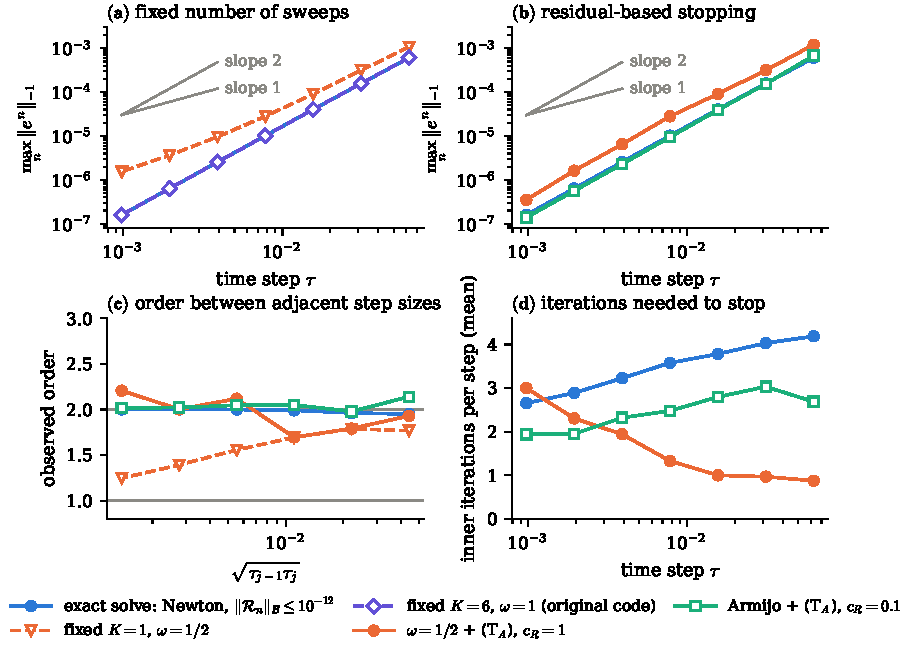
\includegraphics[width=\linewidth]{../figs/fig1_accuracy.pdf}
\caption{Accuracy (manufactured solution, $(0,1)^2$, $N=48$, $\eps=0.1$, $A=1$, $T=1$). (a,b)~$\max_n\nrm{e^n}_{-1}$ against $\tau$, fixed sweep counts (a) and residual-based stopping (b); exact solve (Newton, $\nB{\Rn}\le10^{-12}$) in both. (c)~$\log(e_{j-1}/e_j)/\log(\tau_{j-1}/\tau_j)$ at $\sqrt{\tau_{j-1}\tau_j}$. (d)~Mean inner iterations per step; values below one mean that the predictor passes (T$_A$) in some steps. All ten variants are in \cref{tab:accuracy}.}\label{fig:accuracy}
\end{figure}

\begin{table}[tbp]
\caption{Accuracy test, all inner-solve variants: observed orders $p_j$, error at $\tau_{10}=2^{-10}$ relative to the exact solve, and range over $\tau$ of the mean number of inner iterations per step.}\label{tab:accuracy}
\centering\scriptsize\setlength{\tabcolsep}{3.5pt}
\begin{tabular}{lcccccccc}
\toprule
& \multicolumn{6}{c}{$p_j=\log_2(e_{j-1}/e_j)$, $\tau_j=2^{-j}$} & $e_{10}/e^{\rm ex}_{10}$ & mean it.\\
\cmidrule(lr){2-7}
inner solve & $j=5$ & $j=6$ & $j=7$ & $j=8$ & $j=9$ & $j=10$ & & \\
\midrule
Newton, $\nB{\Rn}\le10^{-12}$ (exact) & 1.95 & 1.96 & 1.99 & 2.00 & 2.00 & 2.00 & 1.00 & 2.65--4.19\\
$\omega=1$, $K=1$ & 1.88 & 1.97 & 1.99 & 2.00 & 2.00 & 2.00 & 0.84 & 1.00--1.00\\
$\omega=1$, $K=2$ & 2.08 & 1.96 & 2.00 & 2.01 & 2.01 & 2.01 & 1.00 & 2.00--2.00\\
$\omega=1$, $K=6$ (original code) & 1.95 & 1.96 & 1.99 & 2.00 & 2.00 & 2.00 & 1.00 & 6.00--6.00\\
$\omega=\frac12$, $K=1$ & 1.77 & 1.79 & 1.69 & 1.56 & 1.39 & 1.25 & 9.68 & 1.00--1.00\\
$\omega=\frac12$, $K=2$ & 1.96 & 1.86 & 1.83 & 1.72 & 1.57 & 1.40 & 3.86 & 2.00--2.00\\
$\omega=\frac12$, $K=4$ & 1.95 & 1.94 & 1.95 & 1.92 & 1.85 & 1.73 & 1.56 & 4.00--4.00\\
$\omega=\frac12$ + (T$_A$), $c_R=1$ & 1.93 & 1.79 & 1.70 & 2.12 & 2.00 & 2.21 & 2.21 & 0.88--3.00\\
Armijo + (T$_A$), $c_R=1$ & 1.82 & 2.31 & 2.07 & 2.80 & 2.00 & 2.00 & 0.84 & 0.62--1.00\\
Armijo + (T$_A$), $c_R=0.1$ & 2.14 & 1.98 & 2.05 & 2.05 & 2.02 & 2.02 & 0.88 & 1.94--3.03\\
\bottomrule
\end{tabular}

\end{table}

\Cref{fig:accuracy,tab:accuracy} are consistent with \eqref{eq:fixedKres} and \cref{prop:linfixed}:
\begin{itemize}
\item $\omega=\frac12$, fixed $K=1,2,4$: $p_j$ decreases to $1.25,1.40,1.73$ at $j=10$; $e_{10}/e^{\rm ex}_{10}=9.7,3.9,1.6$.
\item $\omega=1$, fixed $K$: $p_j\in[1.88,2.08]$; $e_{10}/e^{\rm ex}_{10}=0.84,1.00,1.00$ for $K=1,2,6$ (leading term of \eqref{eq:fixedKres} vanishes).
\item $\omega=\frac12$ + (T$_A$): $p_j\in[1.70,2.21]$, $e_{10}/e^{\rm ex}_{10}=2.21$, $0.88$--$3.00$ iterations. Armijo + (T$_A$): $c_R=1$, $p_j\in[1.82,2.80]$; $c_R=0.1$, $p_j\in[1.98,2.14]$, ratio $0.88$--$1.12$ over $\tau$.
\item The isolated $p_8=2.80$ (Armijo, $c_R=1$) coincides with the change of the mean iteration count from $0.97$ to $1.00$; we attribute it to the switch between accepting the predictor and one iteration.
\end{itemize}
Spatial accuracy ($\phi=0.4\cos t\sin(2\pi x)e^{\cos(2\pi y)}$, $\tau=10^{-4}$, $T=0.01$, exact solves): discrete $L^2$ errors $4.0\cdot10^{-3}$, $2.6\cdot10^{-5}$, $2.4\cdot10^{-7}$, $3.5\cdot10^{-9}$ for $N=8,12,16,20$, and $2.8\cdot10^{-9}$ for $24\le N\le64$ (an $N$-independent floor, attributed to the time discretization).

\subsection{Robustness and cost}\label{sec:num-robust}
\emph{One hard step} (\cref{fig:robust}(a,b)): step $n=20$ ($t=0.08$, end of the spinodal stage, $\max|\phi^n|\approx1.05$) of the problem $[0,6.4)^2$, $N=256$, $\eps=0.02$, $\tau=0.004$, seed~$1$; common history from Newton; runs to $\nB{\Rn}\le10^{-12}$ or $150$ iterations. Transforms to acceptance (practical / tight $10^{-10}$):

\smallskip
\centerline{\small\begin{tabular}{lcccc}
\toprule
& linear $\omega=1$ & relaxed $\omega=\frac12$ & Armijo & Newton--PCG\\
\midrule
$A=0$, $\theta_N=1.83$ & diverges ($\nB{\Rn}:0.20\to3\cdot10^{17}$) & 53 / 149 & 31 / 69 & 35 / 59\\
$A=2$, $\theta_N=0.39$ & 115 / 255 & 33 / 65 & 25 / 47 & 27 / 43\\
\bottomrule
\end{tabular}}
\smallskip

\noindent\emph{Whole runs} (\cref{tab:solver}, $T=1$): the unrelaxed iteration diverges in $4$ of $6$ settings. \Cref{cor:linear} guarantees convergence if $M_0<(2/(3\theta_N))^{1/2}=0.85,0.60,0.43$ ($A=0$) and $1.44,1.30,1.23$ ($A=2$) for $\tau=0.001,0.004,0.016$; the divergent runs fail after the amplitude exceeds these values (the condition is sufficient, not necessary). $\omega=\frac12$ fails only for $A=0$, $\tau=0.016$, where $\frac12>2/(1+q_0)$ as soon as $M_0>0.74$. Armijo and Newton converge in all settings.

\begin{figure}[tbp]
\centering
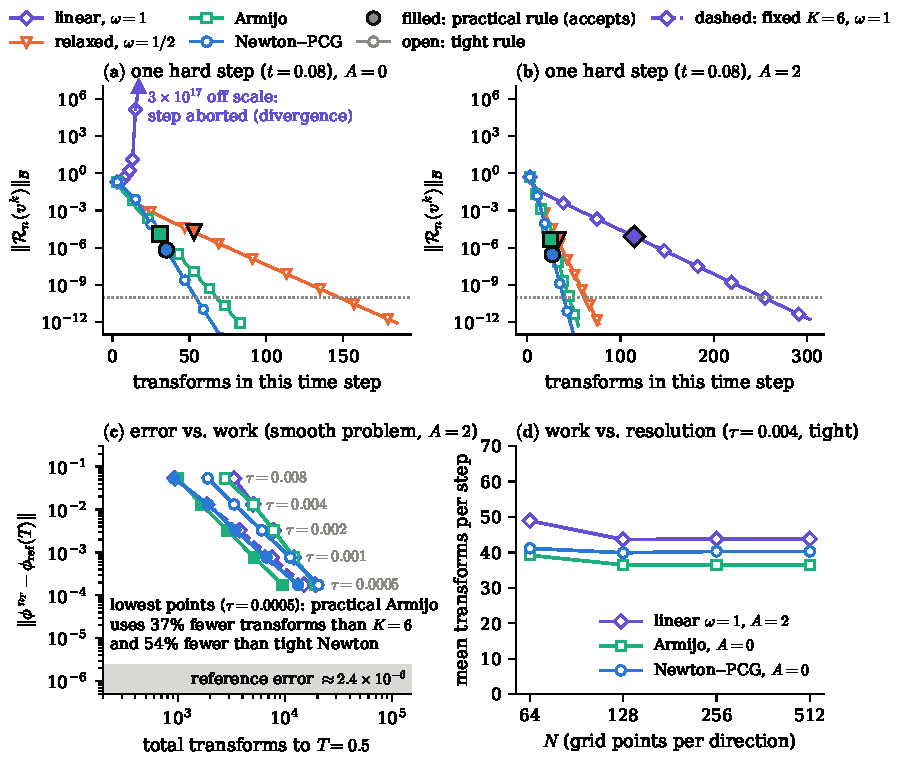
\includegraphics[width=\linewidth]{../figs/fig2_robustness.pdf}
\caption{Robustness and cost. (a,b)~$\nB{\Rn(v^k)}$ against cumulative transforms in step $n=20$ ($t=0.08$) of $[0,6.4)^2$, $N=256$, $\eps=0.02$, $\tau=0.004$, seed~$1$; large filled markers: practical acceptance; dotted line: $10^{-10}$. In (a) the last residual of the unrelaxed iteration, $3\cdot10^{17}$, lies above the range (triangle); the step is then aborted. (c)~Discrete $L^2$ error at $T=0.5$ against total transforms for the smooth interface problem ($[0,2)^2$, $N=128$, $\eps=0.04$, $A=2$, $\tau=0.008,\dots,0.0005$), reference $\tau=6.25\cdot10^{-5}$, Newton to $10^{-12}$; shaded: below the Richardson estimate $2.4\cdot10^{-6}$ of the reference error; annotation: savings at the smallest $\tau$ from the unrounded counts ($9444$ against $15000$ and $20412$). (d)~Mean transforms per step against $N$ ($[0,6.4)^2$, $\eps=0.04$, $\tau=0.004$, $T=1$, tight rule, modes $|k_i|\le16$).}\label{fig:robust}
\end{figure}

\begin{table}[tbp]
\caption{$[0,6.4)^2$, $N=256$, $\eps=0.02$, seed~$1$, $T=1$: mean inner iterations (it) and transforms (FFT) per step; ``div.'' divergence. $\theta_N=0.91,1.83,3.65$ ($A=0$), $0.32,0.39,0.44$ ($A=2$) for $\tau=0.001,0.004,0.016$.}\label{tab:solver}
\centering\scriptsize\setlength{\tabcolsep}{3pt}
\begin{tabular}{llrrrrrrrrrrrr}
\toprule
& & \multicolumn{4}{c}{$\tau=0.001$} & \multicolumn{4}{c}{$\tau=0.004$} & \multicolumn{4}{c}{$\tau=0.016$}\\
\cmidrule(lr){3-6}\cmidrule(lr){7-10}\cmidrule(lr){11-14}
& & \multicolumn{2}{c}{$A=0$} & \multicolumn{2}{c}{$A=2$} & \multicolumn{2}{c}{$A=0$} & \multicolumn{2}{c}{$A=2$} & \multicolumn{2}{c}{$A=0$} & \multicolumn{2}{c}{$A=2$}\\
stop & method & it & FFT & it & FFT & it & FFT & it & FFT & it & FFT & it & FFT\\
\midrule
\multirow{4}{*}{\shortstack[l]{$\nB{\Rn}\le10^{-10}$}} & linear, $\omega=1$ & \multicolumn{2}{c}{div.} & 18.8 & 41 & \multicolumn{2}{c}{div.} & 41.0 & 85 & \multicolumn{2}{c}{div.} & \multicolumn{2}{c}{div.}\\
 & relaxed, $\omega=\frac12$ & 22.4 & 48 & 23.1 & 49 & 83.7 & 170 & 26.8 & 57 & \multicolumn{2}{c}{div.} & 30.2 & 63\\
 & Armijo & 15.0 & 33 & 18.8 & 41 & 28.1 & 59 & 18.6 & 40 & 57.2 & 117 & 19.8 & 43\\
 & Newton--PCG & 3.4 & 36 & 3.2 & 27 & 4.4 & 54 & 4.0 & 34 & 5.5 & 81 & 4.8 & 41\\
\midrule
\multirow{4}{*}{\shortstack[l]{(T$_E$)+(T$_A$)}} & linear, $\omega=1$ & \multicolumn{2}{c}{div.} & 8.2 & 19 & \multicolumn{2}{c}{div.} & 16.0 & 35 & \multicolumn{2}{c}{div.} & \multicolumn{2}{c}{div.}\\
 & relaxed, $\omega=\frac12$ & 11.1 & 25 & 11.7 & 26 & 21.6 & 46 & 11.2 & 25 & \multicolumn{2}{c}{div.} & 10.5 & 24\\
 & Armijo & 7.2 & 17 & 8.2 & 19 & 10.5 & 24 & 8.1 & 19 & 17.2 & 37 & 7.2 & 17\\
 & Newton--PCG & 2.0 & 22 & 2.1 & 18 & 2.2 & 27 & 2.2 & 20 & 2.6 & 39 & 2.3 & 22\\
\bottomrule
\end{tabular}

\end{table}

\noindent\emph{Work at measured accuracy} (\cref{fig:robust}(c)). The random problem is unsuitable: halving $\tau$ changes it by $O(1)$ (\cref{sec:num-bench}), reflecting $e^{CT\eps^{-2}}$ in \cref{thm:error}. We use, on $[0,2)^2$ with $L=2$,
\[
\phi^0=\tanh\frac{\max\{d_\star,d_1,d_2\}}{\sqrt2\eps},\qquad d_\star=0.22L+0.04L\cos6\vartheta-r,\qquad d_i=0.11L-|x-c_i|,
\]
with polar coordinates $(r,\vartheta)$ about $(0.32L,0.5L)$ (a six-lobed star), $c_1=(0.7L,0.36L)$, $c_2=(0.7L,0.64L)$; the circles merge and the star relaxes; $\nrm{\phi_{\rm ref}(T)}=1.87$. All six variants have the same error at each $\tau$ (spread $<0.05\%$), with order $2.01$--$2.13$, and none fails. Transforms relative to the original code ($\omega=1$, $K=6$): practical Armijo $1.08,0.88,0.77,0.69,0.63$ for $\tau=0.008,\dots,0.0005$; practical Newton $0.88$--$1.02$; tight variants $1.27$--$3.58$. Against the same method run to the tight tolerance, the practical rule uses $50.5$--$67.3\%$ (Armijo) and $35.4$--$51.5\%$ (Newton) fewer transforms. The original code is as accurate here ($A=2$, smooth data) but diverges for $A=0$ (panel (a)).

\noindent\emph{Mesh} (\cref{fig:robust}(d)): from $N=64$ to $512$ the transforms per step change $49\to44$ (linear, $A=2$), $39\to36$ (Armijo, $A=0$), $41\to40$ (Newton, $A=0$), consistent with the $N$-independence of $\theta_N$ in \cref{thm:local,thm:newton}.

\subsection{Reliability of the a posteriori bound}\label{sec:num-estimator}
$[0,3.2)^2$, $N=128$, $\eps=0.02$, $A=2$, $\tau=0.004$, seed~$3$; reference step solutions by Newton to $\nB{\Rn}\le10^{-13}$. (a) $739$ iterates (first $15$ of $\omega=1$ and $\omega=\frac12$ at $n=0,10,\dots,240$): $\nBi{v-\phi^{n+1}}/\nB{\Rn(v)}\in[0.589,0.9996]$ ($\omega=1$: $\ge0.589$; $\omega=\frac12$: $\ge0.654$), against the guaranteed interval $[1/(1+q_{\max}),1]=[0.448,1]$ of \eqref{eq:apost} with $q_{\max}=1.23$. (b) First iterate with $\nB{\Rn}\le\mathrm{tol}$, $\mathrm{tol}=10^{-2},\dots,10^{-10}$, four methods, $n=5,15,\dots,245$: $500$ accepted iterates, error/tol $\in[2.2\cdot10^{-3},0.974]$, no violation.

\begin{figure}[tbp]
\centering
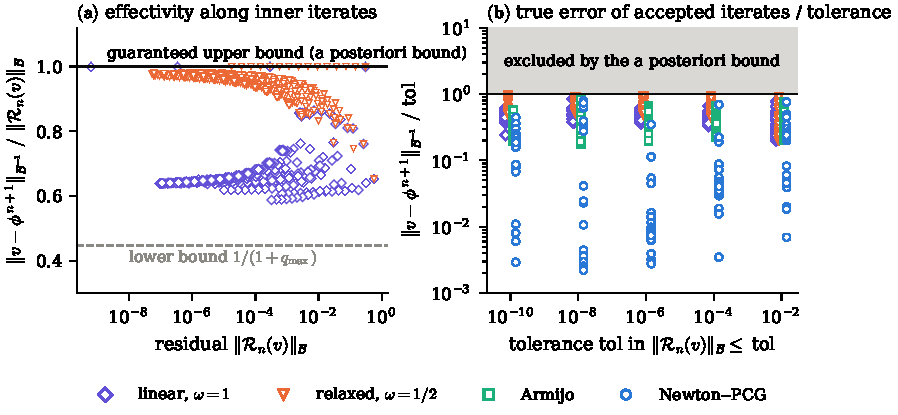
\includegraphics[width=\linewidth]{../figs/fig3_estimator.pdf}
\caption{A posteriori bound ($[0,3.2)^2$, $N=128$, $\eps=0.02$, $A=2$, $\tau=0.004$, seed~$3$; references by Newton to $10^{-13}$). (a)~$\nBi{v-\phi^{n+1}}/\nB{\Rn(v)}$ for $739$ iterates; dashed: $1/(1+q_{\max})$ with $q_{\max}=\max q(M_v)$, $M_v$ as in \cref{thm:apost}, $\theta_N=0.39$. (b)~True error/tolerance for the first accepted iterate ($500$ iterates, methods offset horizontally); the shaded region is excluded by \cref{thm:apost}.}\label{fig:estimator}
\end{figure}

\subsection{Coarsening benchmark}\label{sec:num-bench}
The problem of \cite{ChengWangWiseYue2016}: $[0,12.8)^2$, $N=512$, $\eps=0.02$, $A=0$, $\tau=0.004$, $T=10$, seed~$1$ (mean $-8.7\cdot10^{-5}$); practical and tight solvers in lockstep, i.e.\ two solvers of the \emph{same} fully discrete problem. The trajectory is not converged in time: the fastest linear mode has rate $\lambda_{\max}=(4\eps^2)^{-1}=625$, $\tau\lambda_{\max}=2.5$, and halving $\tau$ changes the solution by $8.7$ ($t=0.2$) and $12.2$ ($t=1$) in $L^2$; the energies $E+|\Omega|/4$ of the $\tau$ and $\tau/2$ runs differ by $0.4\%$ and $0.8\%$.

\begin{figure}[tbp]
\centering
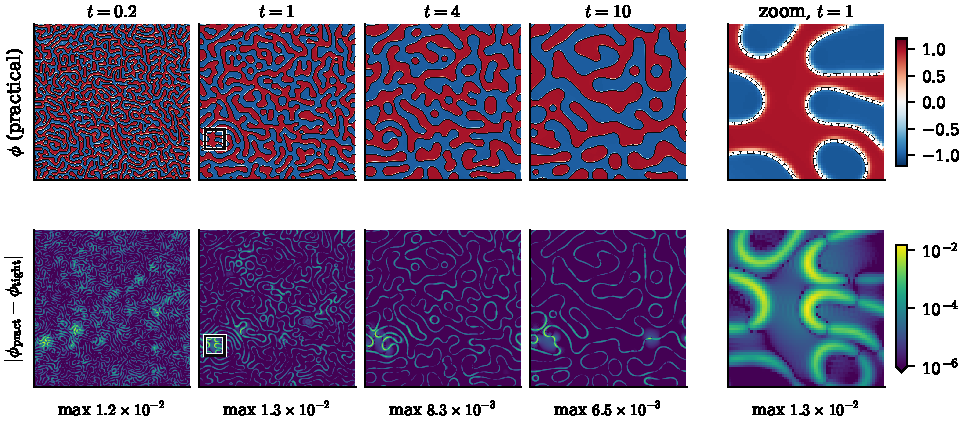
\includegraphics[width=\linewidth]{../figs/fig4_coarsening.pdf}
\caption{Coarsening benchmark ($[0,12.8)^2$, $N=512$, $\eps=0.02$, $A=0$, $\tau=0.004$, seed~$1$); both solvers solve the same discrete problem, which is not converged in $\tau$. Columns 1--4: full domain at $t=0.2,1,4,10$; column 5: the $1.6\times1.6$ box ($64^2$ points) marked at $t=1$, centred on the largest difference. Top: practical $\phi$, limits $[-1.2,1.2]$ (all values in $[-1.149,1.040]$); black: tight zero level set; white dashed (column 5): practical zero level set. Bottom: $|\phi_{\rm pract}-\phi_{\rm tight}|$ on $[10^{-6},1.5\cdot10^{-2}]$ (contains every maximum, stated beneath).}\label{fig:coarsening}
\end{figure}

\begin{figure}[tbp]
\centering
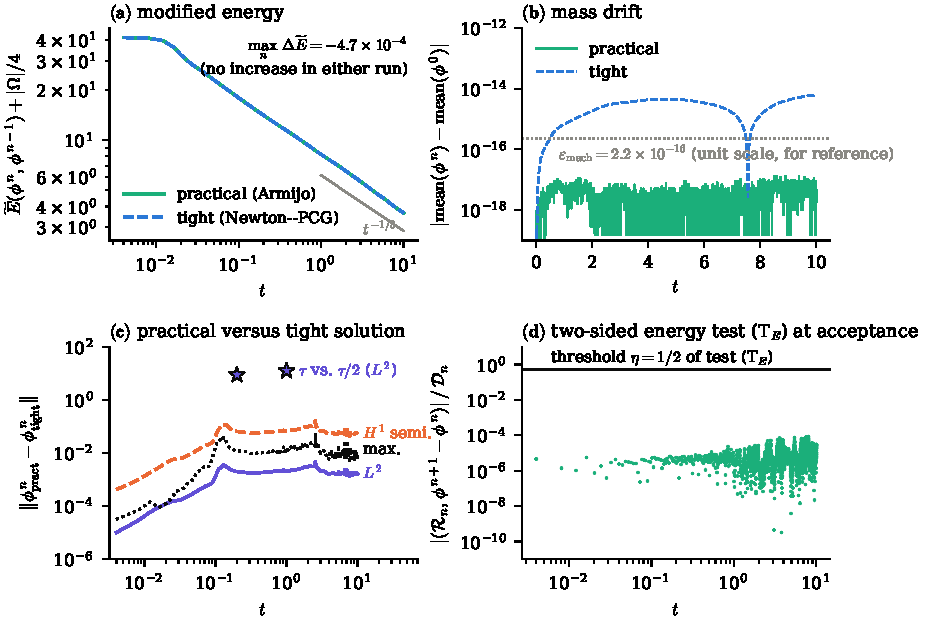
\includegraphics[width=\linewidth]{../figs/fig5_structure.pdf}
\caption{Structure on the benchmark of \cref{fig:coarsening}; practical solid (green), tight dashed (blue). (a)~$\Et(\phi^n,\phi^{n-1})+|\Omega|/4$; grey: slope $-\frac13$. (b)~$|\mean(\phi^n)-\mean(\phi^0)|$; dotted: machine epsilon $2.2\cdot10^{-16}$ as a unit-scale reference, not a bound. (c)~Practical minus tight in $L^2$, $H^1$ seminorm and maximum norm; stars: $L^2$ difference of tight solutions with $\tau$ and $\tau/2$. (d)~$|\ip{\Rn(v)}{v-\phi^n}|/\Dn(v)$ at acceptance; the two-sided test requires $\le\eta=\frac12$ and is stronger than needed for decay (\cref{rem:onesided}).}\label{fig:structure}
\end{figure}

Practical: $7.3$ iterations per step (max $18$), $17.6$ transforms; tight: $3.6$ Newton iterations (max $6$), $45.0$ transforms; all steps accepted with $\nrm{\rho^n}\le1.6\cdot10^{-5}=c_R\tau^2$. Differences (\cref{fig:coarsening,fig:structure}): snapshot median $\le1.5\cdot10^{-6}$, 99th percentile $\le2.2\cdot10^{-4}$, maximum $\le1.35\cdot10^{-2}$; over the run $\max_n\nrm{\phi_{\rm p}^n-\phi_{\rm t}^n}=4.7\cdot10^{-3}$ ($t\approx2.5$; relative $\le4\cdot10^{-4}$ since $\nrm{\phi}\in[11.0,12.4]$), $H^1$ seminorm $<0.16$, maximum norm $<0.05$. $\Et$ decreases at every step of both runs (largest change $-4.7\cdot10^{-4}$; relative difference of $\Et+|\Omega|/4$ between runs $\le1.7\cdot10^{-5}$); between $t=1$ and $10$, $\Et+|\Omega|/4\sim t^{-0.36}$, close to $t^{-1/3}$ \cite{KohnOtto2002}. Maximal mass drift $1.3\cdot10^{-17}$ (practical) and $6.0\cdot10^{-15}$ (tight). (T$_E$) ratio $\le7.9\cdot10^{-5}$ (median $6\cdot10^{-6}$).

\subsection{Interface evolution: merger and Ostwald ripening}\label{sec:num-interface}
Protocol: (1) tight solutions for $\tau=8\tau_0,\dots,\tau_0$ ($\tau_0=2.5\cdot10^{-4}$ star, $5\cdot10^{-4}$ droplets); (2) $N$ against $2N$; (3) the reported observables; (4) practical and tight solvers in lockstep at the production resolution, same data and output times, constant $\tau$. Observables (\cref{app:observables}): the number of components of $\{\phi>0\}$ (periodic, 4-connectivity), a merger time being its first decrease; the interface-displacement proxy $\delta_\Gamma(a,b)=\nrm{a-b}_{L^1}/(2|\Gamma_b|)$, which equals the mean normal displacement to leading order for equal profiles and nearby interfaces but is not a geometric measurement or bound in general; the equivalent radius $R_j=(\mathcal A_j/\pi)^{1/2}$ from the marching-squares zero contour nearest to droplet $j$'s previous centroid (within $0.15$), a disappearance time being the first step without such a contour.

\begin{table}[tbp]
\caption{Resolution study (tight solver). Star: $\delta_\Gamma$ against $N=128$, $\tau=2.5\cdot10^{-4}$ at $t=0.1,0.25,0.5$, and merger times. Droplets: largest difference of the radii at $t=0.15,1,2$ against the run in column~3, and disappearance times $t_1,t_2$. Production resolutions~$^\ast$.}\label{tab:resolution}
\centering\scriptsize\setlength{\tabcolsep}{4pt}
\begin{tabular}{lllcccc}
\toprule
\multicolumn{7}{l}{\emph{Star and two circles} ($A=2$, $T=0.5$): displacement proxy $\delta_\Gamma(t)$ against $N=128$, $\tau=2.5\cdot10^{-4}$}\\
$N$ & $\tau$ & & $\delta_\Gamma(0.1)$ & $\delta_\Gamma(0.25)$ & $\delta_\Gamma(0.5)$ & $t_{m,1}$, $t_{m,2}$\\
\midrule
128 & $0.002$ &  & $8.0\cdot10^{-4}$ & $1.5\cdot10^{-3}$ & $3.3\cdot10^{-4}$ & $0.03400$, $0.1980$\\
128 & $0.001$ & $^\ast$ & $1.9\cdot10^{-4}$ & $3.4\cdot10^{-4}$ & $7.5\cdot10^{-5}$ & $0.03000$, $0.1940$\\
128 & $0.0005$ &  & $3.7\cdot10^{-5}$ & $6.6\cdot10^{-5}$ & $1.4\cdot10^{-5}$ & $0.02900$, $0.1935$\\
128 & $0.00025$ & ref. & -- & -- & -- & $0.02875$, $0.1930$\\
256 & $0.00025$ &  & $3.1\cdot10^{-5}$ & $3.4\cdot10^{-5}$ & $1.6\cdot10^{-5}$ & $0.02850$, $0.1930$\\
\midrule
\multicolumn{7}{l}{\emph{Unequal droplets} ($A=0$, $T=2$): radii at $t=0.15,1,2$ against the run in column 3}\\
$N$ & $\tau$ & against & \multicolumn{3}{c}{$\max_{j,k}|R_j(t_k)-R_j^{\rm cmp}(t_k)|$} & $t_1$, $t_2$\\
\midrule
256 & $0.004$ & $N=256$, $\tau=0.001$ & \multicolumn{3}{c}{$1.3\cdot10^{-3}$} & $0.2040$, $1.5560$\\
256 & $0.002$ & $N=256$, $\tau=0.001$ & \multicolumn{3}{c}{$5.3\cdot10^{-5}$} & $0.2000$, $1.5540$\\
256 & $0.001$ & $^\ast$ & \multicolumn{3}{c}{--} & $0.1990$, $1.5520$\\
256 & $0.0005$ & $N=256$, $\tau=0.001$ & \multicolumn{3}{c}{$1.3\cdot10^{-5}$} & $0.1985$, $1.5520$\\
128 & $0.0005$ & $N=256$, $\tau=0.0005$ & \multicolumn{3}{c}{$1.7\cdot10^{-4}$} & $0.1985$, $1.5520$\\
512 & $0.001$ & $N=256$, $\tau=0.001$ & \multicolumn{3}{c}{$4.2\cdot10^{-5}$} & $0.1990$, $1.5520$\\
\bottomrule
\end{tabular}

\end{table}

\emph{Merger} (\cref{fig:star}): the problem of \cref{fig:robust}(c), $[0,2)^2$, $\eps=0.04$, $A=2$, $T=0.5$; the circles merge at $t\approx0.029$, the relaxed star joins them through a neck at $t\approx0.193$. \Cref{tab:resolution}: $\delta_\Gamma$ decreases at second order in $\tau$; at $N=128$, $\tau=10^{-3}$, $\delta_\Gamma\le3.4\cdot10^{-4}\approx h/46$ and the merger times differ from the reference by $1.25\tau$ and $\tau$; $2N$ gives $\delta_\Gamma\le3.4\cdot10^{-5}$. Practical versus tight: identical merger steps ($0.030$, $0.194$); $\delta_\Gamma\le8.3\cdot10^{-8}$ at the output times against $6.1\cdot10^{-5}$--$2.8\cdot10^{-4}$ for $\tau$ versus $\tau/2$ (a factor $700$--$4600$ in $\delta_\Gamma$); fields differ by $\le8.8\cdot10^{-7}$ in $L^2$ and $\le6.1\cdot10^{-6}$ pointwise, largest at the neck; $5140$ transforms (practical Armijo) against $11180$ (tight Newton--PCG), $54.0\%$ fewer. Cost peaks in the first steps and around the second merger, briefly for the tight solver ($t\approx0.19$--$0.24$), longer for the practical one ($t\approx0.17$--$0.33$).

\begin{figure}[tbp]
\centering
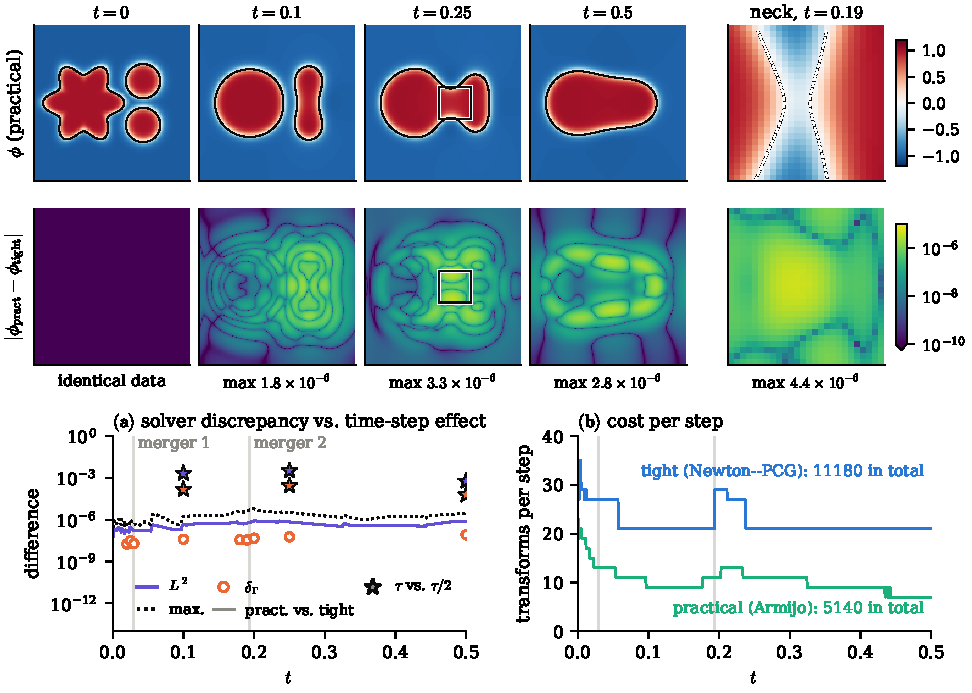
\includegraphics[width=\linewidth]{../figs/fig6_star.pdf}
\caption{Merger ($[0,2)^2$, $N=128$, $\eps=0.04$, $A=2$, $\tau=10^{-3}$). Top: practical $\phi$ at $t=0,0.1,0.25,0.5$, limits $[-1.2,1.2]$ (values in $[-1.019,1.044]$), tight zero level set black; column~5: the box marked at $t=0.25$ ($0.41^2$, $26^2$ points) at $t=0.19$, practical zero level set white dashed. Bottom: $|\phi_{\rm pract}-\phi_{\rm tight}|$ on $[10^{-10},10^{-5}]$ (contains every maximum). (a)~Practical minus tight: $L^2$ (line), maximum norm (dotted), $\delta_\Gamma$ (circles); stars: the same $L^2$ and $\delta_\Gamma$ for tight $\tau=10^{-3}$ against $5\cdot10^{-4}$; vertical lines: merger times. (b)~Transforms per step.}\label{fig:star}
\end{figure}

\emph{Ostwald ripening} (\cref{fig:droplets}): $[0,2)^2$, $\eps=0.04$, $A=0$, droplets ($\phi=1$ inside) of radii $0.16,0.24,0.32$ centred at $(1.00,1.50)$, $(1.45,0.72)$, $(0.58,0.62)$, tanh profiles of the periodic distance, closest interfaces $0.32\approx8\eps$ apart. The smallest droplet disappears at $t\approx0.199$, the middle one at $t\approx1.552$, and $R_3(2)=0.4195$. At $N=256$, $\tau=10^{-3}$ the radii at $t=0.15,1,2$ agree with $\tau/2$ to $1.3\cdot10^{-5}$ and with $N=512$ to $4.2\cdot10^{-5}$; disappearance times agree within one step. Practical versus tight: identical disappearance steps; median $|R_j^{\rm p}-R_j^{\rm t}|\le2.4\cdot10^{-7}$ against a median time-step effect $\ge1.5\cdot10^{-6}$; maximum $7.4\cdot10^{-5}$ ($R_2$, $t=1.551$) against a time-step effect of $2.2\cdot10^{-3}$ there; $\delta_\Gamma\le3.4\cdot10^{-7}$ at the output times; $\le4.3\cdot10^{-5}$ in $L^2$ over the run; $14492$ transforms (practical Armijo) against $43278$ (tight Newton--PCG), $66.5\%$ fewer.

\begin{figure}[tbp]
\centering
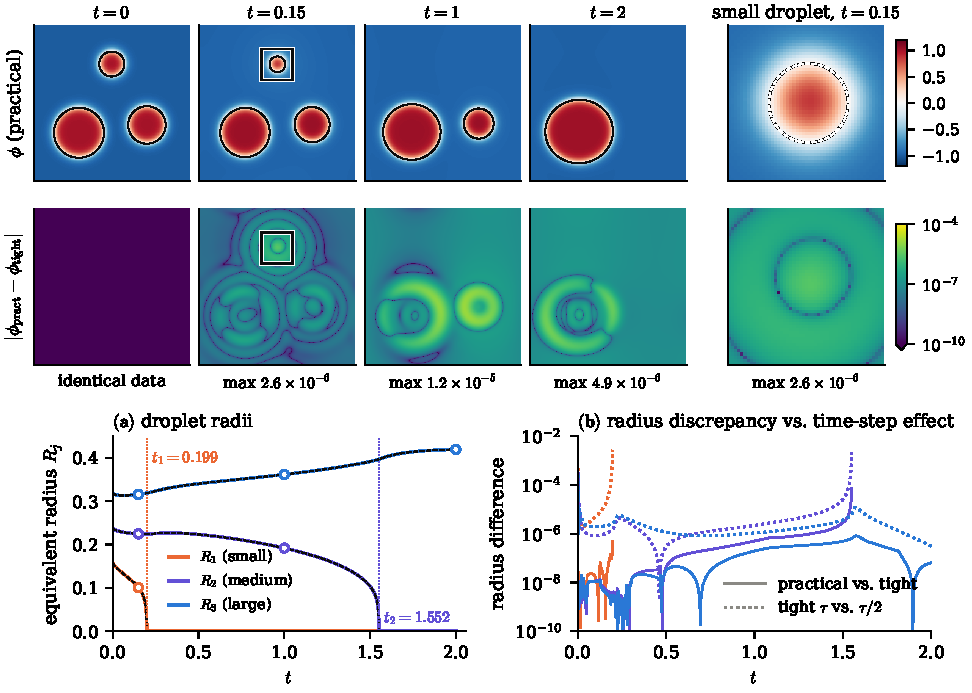
\includegraphics[width=\linewidth]{../figs/fig7_droplets.pdf}
\caption{Ostwald ripening ($[0,2)^2$, $N=256$, $\eps=0.04$, $A=0$, $\tau=10^{-3}$). Top: practical $\phi$ at $t=0,0.15,1,2$, limits $[-1.2,1.2]$ (values in $[-1.000,1.041]$), tight zero level set black; column~5: the small droplet at $t=0.15$ (box $0.40^2$, $51^2$ points), practical zero level set white dashed. Bottom: $|\phi_{\rm pract}-\phi_{\rm tight}|$ on $[10^{-10},10^{-4}]$. (a)~$R_j(t)$: practical (coloured), tight (black dashed), tight with $\tau/2$ at the output times (circles); dotted: disappearance times (identical in both runs). (b)~$|R_j^{\rm p}-R_j^{\rm t}|$ (solid) and $|R_j(\tau)-R_j(\tau/2)|$ of the tight solver (dotted); colours as in (a).}\label{fig:droplets}
\end{figure}

\subsection{Nonzero mean, three seeds}\label{sec:num-seeds}
$[0,6.4)^2$, $N=256$, $\eps=0.04$, $A=0$, $\tau=0.002$, $T=5$, $\phi^0=\bar\phi+0.05\,P/\max|P|$ with $\bar\phi=-0.5$ and $P(x)=\sum_{|k_1|,|k_2|\le24}c_ke^{\mathrm i\kappa_k\cdot x}$, $\hat P_0=c_0=0$, $c_{-k}=\overline{c_k}$ (so $P$ is real), $c_k=\frac12(z_k+\overline{z_{-k}})$ with $\mathrm{Re}\,z_k,\mathrm{Im}\,z_k$ independent standard normal (NumPy default generator, seeds $1,2,3$; coefficients stored); $\max|P|$ is taken over the $1024\times1024$ grid for every $N$, so the initial function is the same on all grids (the $N=256$ and $N=512$ data agree at common points to $10^{-16}$). Linearizing \eqref{eq:ch} at $\bar\phi$, $\hat\phi_t=-s(f''(\bar\phi)+\eps^2s)\hat\phi$ with $f''(\bar\phi)=3\bar\phi^2-1=-\frac14$, so $\lambda_{\max}=\max_s s(\frac14-\eps^2s)=(64\eps^2)^{-1}\approx9.8$ and $\tau\lambda_{\max}\approx0.02$.

\begin{figure}[tbp]
\centering
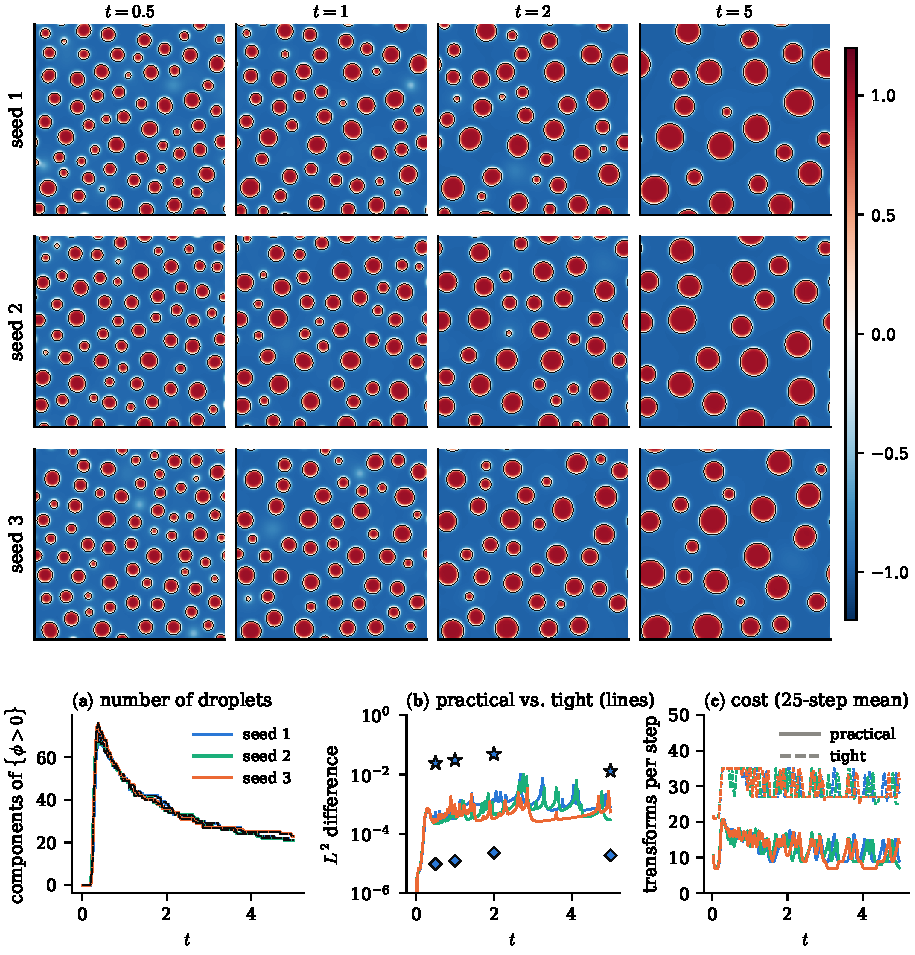
\includegraphics[width=\linewidth]{../figs/figS2_seeds.pdf}
\caption{Nonzero mean ($[0,6.4)^2$, $N=256$, $\eps=0.04$, $A=0$, $\tau=0.002$, $\bar\phi=-0.5$). Top: practical $\phi$ for seeds 1--3 at $t=0.5,1,2,5$, limits $[-1.2,1.2]$ (values in $[-0.980,1.039]$), tight zero level set black. (a)~Components of $\{\phi>0\}$: practical coloured, tight black dashed. (b)~$L^2$ difference practical--tight (lines, colours as in (a)); seed~1, tight: $\tau$ against $\tau/2$ (stars), $N$ against $2N$ (diamonds). (c)~Transforms per step, 25-step moving average: practical solid, tight dashed.}\label{fig:seeds}
\end{figure}

\begin{table}[tbp]
\caption{Seed study (practical Armijo, p, against tight Newton--PCG, t): transforms FFT$_{\rm p}$ / FFT$_{\rm t}$ and the factor FFT$_{\rm t}$/FFT$_{\rm p}$; failures; number of steps (of $2500$) with different droplet counts (largest difference); largest $\delta_\Gamma$ at $t=0.5,1,2,5$; largest $L^2$ difference; largest (T$_E$) ratio; largest mass drift.}\label{tab:seeds}
\centering\scriptsize\setlength{\tabcolsep}{3pt}
\begin{tabular}{lcccccccc}
\toprule
seed & FFT$_{\rm p}$ / FFT$_{\rm t}$ & FFT$_{\rm t}$/FFT$_{\rm p}$ & failures & count differs (max) & $\max_k\delta_\Gamma(t_k)$ & $\max_n\|\phi_p-\phi_t\|$ & (T$_E$) ratio & mass drift\\
\midrule
1 & 31328 / 74300 & 2.37 & 0 & 4 (1) & $1.6\cdot10^{-5}$ & $1.0\cdot10^{-2}$ & $3.1\cdot10^{-4}$ & $4.9\cdot10^{-15}$\\
2 & 31190 / 73616 & 2.36 & 0 & 4 (1) & $1.0\cdot10^{-5}$ & $1.0\cdot10^{-2}$ & $2.9\cdot10^{-4}$ & $2.2\cdot10^{-15}$\\
3 & 30288 / 73752 & 2.44 & 0 & 3 (1) & $1.3\cdot10^{-5}$ & $3.4\cdot10^{-3}$ & $3.3\cdot10^{-4}$ & $6.8\cdot10^{-15}$\\
\bottomrule
\end{tabular}

\end{table}

\emph{Refinement (seed~1 only, tight).} $N=512$: $L^2$ difference $\le2.3\cdot10^{-5}$, $\delta_\Gamma\le5.1\cdot10^{-7}$ at $t=0.5,1,2,5$, same droplet count at every step. $\tau/2$: $L^2$ difference $1.3\cdot10^{-2}$--$4.8\cdot10^{-2}$, $\delta_\Gamma=3.0\cdot10^{-4}$--$5.2\cdot10^{-4}$; counts equal at the output times ($65,50,38,21$) but different at $148$ of $2500$ steps (by up to $4$). Event timing is therefore not converged to one step at $\tau=0.002$.

\emph{Practical versus tight (all seeds; \cref{fig:seeds,tab:seeds}).} No failures (practical $\le9$ iterations, tight $\le4$ Newton iterations, cap $60$); $\Et$ decreases at every step of all six runs; counts rise from $0$ to $67$--$76$ at $t\approx0.35$ and coarsen to $21$--$23$; counts differ at $3$--$4$ of $2500$ steps, by one, against $148$ for $\tau/2$; $\delta_\Gamma\le1.6\cdot10^{-5}$ at the output times ($20$--$63$ times less than the $\tau/2$ effect, seed~1); the largest $L^2$ differences ($1.0\cdot10^{-2}$, $1.0\cdot10^{-2}$, $3.4\cdot10^{-3}$ at $t=2.68,2.75,2.86$) occur at or one step after a droplet removal that happens one step earlier in one run, the median being below $10^{-3}$; $57.6$--$58.9\%$ fewer transforms (practical Armijo against tight Newton--PCG).

\subsection{Synthesis and concluding remarks}\label{sec:conclusion}
\begin{table}[tbp]
\caption{Practical rule with Armijo inner method (p) versus tightly converged Newton--PCG (t) on all lockstep runs: steps, total transforms, saving, topological events (merger or disappearance steps; for the seeds, steps with different droplet counts), largest $L^2$ difference, largest (T$_E$) ratio and mass drift. $\Et$ decreased at every step of every run.}\label{tab:summary}
\centering\scriptsize\setlength{\tabcolsep}{3pt}
\begin{tabular}{lrrrrlccc}
\toprule
run & steps & FFT$_{\rm p}$ & FFT$_{\rm t}$ & fewer & events & $\max_n\nrm{\phi_{\rm p}^n-\phi_{\rm t}^n}$ & (T$_E$) ratio & mass drift\\
\midrule
labyrinth, $512^2$, $\tau=0.004$ & 2500 & 43892 & 112406 & 61.0\% & -- & $4.7\cdot10^{-3}$ & $7.9\cdot10^{-5}$ & $6.0\cdot10^{-15}$\\
merger, $128^2$, $\tau=10^{-3}$ & 500 & 5140 & 11180 & 54.0\% & same & $8.8\cdot10^{-7}$ & $6.3\cdot10^{-6}$ & $1.7\cdot10^{-15}$\\
ripening, $256^2$, $\tau=10^{-3}$ & 2000 & 14492 & 43278 & 66.5\% & same & $4.3\cdot10^{-5}$ & $6.3\cdot10^{-5}$ & $3.7\cdot10^{-15}$\\
$\bar\phi=-0.5$, seed 1, $256^2$, $\tau=0.002$ & 2500 & 31328 & 74300 & 57.8\% & 4/2500 & $1.0\cdot10^{-2}$ & $3.1\cdot10^{-4}$ & $4.9\cdot10^{-15}$\\
$\bar\phi=-0.5$, seed 2, $256^2$, $\tau=0.002$ & 2500 & 31190 & 73616 & 57.6\% & 4/2500 & $1.0\cdot10^{-2}$ & $2.9\cdot10^{-4}$ & $2.2\cdot10^{-15}$\\
$\bar\phi=-0.5$, seed 3, $256^2$, $\tau=0.002$ & 2500 & 30288 & 73752 & 58.9\% & 3/2500 & $3.4\cdot10^{-3}$ & $3.3\cdot10^{-4}$ & $6.8\cdot10^{-15}$\\
\bottomrule
\end{tabular}

\end{table}

\Cref{tab:summary} collects the lockstep comparisons: the practical rule (Armijo) used $54$--$67\%$ fewer transforms than tight Newton--PCG, reproduced merger and disappearance steps, matched droplet radii to $7.4\cdot10^{-5}$ and droplet counts at the output times, and kept $\Et$ decreasing, as \cref{thm:energysafe} guarantees. The unrelaxed iteration diverged in regimes not covered by \cref{cor:linear}, and fixed relaxed sweeps lost order, consistent with \eqref{eq:fixedKres} and \cref{prop:linfixed}; globalized methods stopped by \cref{alg:step} avoided both.

The arguments of \cref{sec:scheme,sec:solver} use only convexity of the implicit part and the constant-coefficient preconditioner, and should extend to other secant and convex-splitting schemes, BDF2 variants and finite-difference discretizations. Error bounds polynomial in $\eps^{-1}$ and logarithmic potentials, where maximum-norm control must be replaced by separation from the singular values, need further ideas.

\medskip{\sloppy\noindent\textbf{Code and data.} The archive \texttt{ch\_inner\_iterations\_submission.zip} contains the solver (\texttt{code/chsolver.py}), the simulation scripts (\texttt{experiments.py}, \texttt{fig\_experiments.py}, \texttt{fig\_experiments2.py}), the raw data (\texttt{data/}), the diagnostics (\texttt{diagnostics.py}, which writes every number quoted in \cref{sec:numerics} to \texttt{data/summary.json}) and the plotting script. From the stored data, all figures and tables are regenerated by \texttt{python3 diagnostics.py} followed by \texttt{python3 make\_figures.py 1 2 3 4 5 6 7 S2 tables}; the commands that rerun each simulation are listed in \texttt{code/README.md}.\par}

\appendix
\section{Auxiliary proofs and implementation}\label{app}

\subsection{Discrete Sobolev inequality}\label{app:sobolev}
\begin{proof}[Proof of \cref{lem:discrete}(c)]
For $f\in\Vo$ and every grid point,
\[
|f_{ij}|\le\sum_{k\ne0}|\hat f_k|\le\Big(\sum_ks_k|\hat f_k|^2\Big)^{1/2}\Big(\sum_{k\ne0}s_k^{-1}\Big)^{1/2}=\frac{\nrm{\gradN f}}{L}\cdot\frac L{2\pi}\Big(\sum_{k\ne0}|k|^{-2}\Big)^{1/2}.
\] The shell $\max(|k_1|,|k_2|)=j$ contains at most $8j$ indices, each with $|k|\ge j$, so
\[
\sum_{k\in K_N\setminus\{0\}}|k|^{-2}\le\sum_{j=1}^{N/2}\frac{8j}{j^2}=8\sum_{j=1}^{N/2}\frac1j\le8\Big(1+\ln\frac N2\Big)\le8(1+\ln N),
\]
hence $\nrm f_\infty\le\frac{\sqrt8}{2\pi}(1+\ln N)^{1/2}\nrm{\gradN f}=C_N\nrm{\gradN f}$. In three dimensions the shell has at most $24j^2+2$ indices and the sum is $O(N)$.
\end{proof}

\subsection{Discrete Gronwall inequality}
\begin{lemma}\label{lem:gronwall}
If $y_k\ge0$ and $y_k\le F+\Lambda\tau\sum_{j=0}^{k-1}y_j$ for $0\le k\le K$, then $y_k\le F(1+\Lambda\tau)^k\le Fe^{\Lambda t_k}$.
\end{lemma}

\begin{proof}
$Z_k=F+\Lambda\tau\sum_{j<k}y_j$ satisfies $Z_0=F$ and $Z_{k+1}=Z_k+\Lambda\tau y_k\le(1+\Lambda\tau)Z_k$; and $y_k\le Z_k$.
\end{proof}

\subsection{Projection and interpolation estimates}\label{app:interp}
\begin{lemma}\label{lem:interp}
For $L$-periodic $g$ and $m\ge1$, with $C$ depending on $L$ and $m$ only,
\[
\nrm{I_Ng}_{H^1}\le C\nrm g_{H^2},\qquad \nrm{g-\mathsf P_Ng}_{H^1}+\nrm{g-I_Ng}_{H^1}\le Ch^m\nrm g_{H^{m+1}} .
\]
\end{lemma}

\begin{proof}
Scale $L=2\pi$ and write $\langle q\rangle=(1+|q|^2)^{1/2}$, $q\in\Z^2$. The interpolant has $\widehat{I_Ng}_k=\sum_{\ell\in\Z^2}\hat g_{k+N\ell}$, $k\in K_N$. For $k\in K_N$ and $\ell\ne0$, $|k+N\ell|\ge N|\ell|_\infty-\frac N2\ge\frac N2|\ell|_\infty$, so by weighted Cauchy--Schwarz
\begin{gather*}
\langle k\rangle^2\Big|\sum_\ell\hat g_{k+N\ell}\Big|^2\le\Big\{\langle k\rangle^2\sum_\ell\langle k+N\ell\rangle^{-4}\Big\}\sum_\ell\langle k+N\ell\rangle^4|\hat g_{k+N\ell}|^2,\\
\Big\{\langle k\rangle^2\sum_\ell\langle k+N\ell\rangle^{-4}\Big\}\le1+\big(1+\tfrac{N^2}2\big)\tfrac{16}{N^4}\sum_{\ell\ne0}|\ell|_\infty^{-4}\le C .
\end{gather*}
Summing over the disjoint classes $k+N\Z^2$ gives the first bound. Next, $g-\mathsf P_Ng$ contains only $|q|_\infty\ge\frac N2$, so $\nrm{g-\mathsf P_Ng}_{H^1}^2\le(\frac N2)^{-2m}\sum\langle q\rangle^{2m+2}|\hat g_q|^2$. Since $I_N\mathsf P_Ng=\mathsf P_Ng$, $g-I_Ng=(g-\mathsf P_Ng)-I_N(g-\mathsf P_Ng)$, and with exponent $m+1$,
\[
\nrm{I_N(g-\mathsf P_Ng)}_{H^1}^2\le\sum_{k\in K_N}\Big\{\langle k\rangle^2\!\!\sum_{q\equiv k,\,|q|_\infty\ge N/2}\!\!\langle q\rangle^{-2(m+1)}\Big\}\sum_{q\equiv k}\langle q\rangle^{2(m+1)}|\hat g_q|^2\le CN^{-2m}\nrm g_{H^{m+1}}^2,
\]
because $\{\cdot\}\le(1+\frac{N^2}2)(\frac N2)^{-2(m+1)}\sum_{\ell}\max(1,|\ell|_\infty)^{-2(m+1)}\le CN^{-2m}$ for $m\ge1$.
\end{proof}

\subsection{Proof of \cref{lem:consistency}}\label{app:consistency}
Let $\bar t=\bar t_n=t_{n+1/2}$, $u_j=u(t_j)$, and for $g\in C^3$ use $g(\bar t+\vartheta)=g+\vartheta g'+\frac{\vartheta^2}2g''+\mathcal T_3(\vartheta)$, $\mathcal T_3(\vartheta)=\frac12\int_{\bar t}^{\bar t+\vartheta}(\bar t+\vartheta-r)^2g'''(r)\,dr$, $|\mathcal T_3(\vartheta)|\le\frac{|\vartheta|^3}6\sup|g'''|$. With $t_{n+1}=\bar t+\frac\tau2$, $t_n=\bar t-\frac\tau2$, $t_{n-1}=\bar t-\frac{3\tau}2$, the coefficients of $\vartheta^0,\vartheta^1,\vartheta^2$ give
\begin{align*}
\tfrac1\tau(u_{n+1}-u_n)-u_t(\bar t)&=\tfrac1\tau\big[\mathcal T_3(\tfrac\tau2)-\mathcal T_3(-\tfrac\tau2)\big],&&|\cdot|\le\tfrac{\tau^2}{24}\sup|u_{ttt}|,\\
c_1:=\tfrac34u_{n+1}+\tfrac14u_{n-1}-u(\bar t)&=\tfrac38\tau^2u_{tt}(\bar t)+\varrho_1,&&|\varrho_1|\le\tfrac5{32}\tau^3\sup|u_{ttt}|,\\
c_2:=\tfrac32u_n-\tfrac12u_{n-1}-u(\bar t)&=-\tfrac38\tau^2u_{tt}(\bar t)+\varrho_2,&&|\varrho_2|\le\tfrac5{16}\tau^3\sup|u_{ttt}|,\\
c_3:=u_{n+1}-2u_n+u_{n-1}&=\tau^2u_{tt}(\bar t)+\varrho_3,&&|\varrho_3|\le\tfrac58\tau^3\sup|u_{ttt}|,
\end{align*}
since, e.g.\ for $c_1$: $\frac34\cdot\frac\tau2+\frac14\cdot(-\frac{3\tau}2)=0$, $\frac12(\frac34\cdot\frac{\tau^2}4+\frac14\cdot\frac{9\tau^2}4)=\frac38\tau^2$ and $\frac16(\frac34\cdot\frac18+\frac14\cdot\frac{27}8)\tau^3=\frac5{32}\tau^3$; similarly for $c_2$ ($-\frac34\tau+\frac34\tau=0$, $\frac12(\frac38-\frac98)\tau^2$) and $c_3$ ($\frac\tau2+\tau-\frac{3\tau}2=0$, $\frac12(\frac14-\frac12+\frac94)\tau^2$). For the secant, with $\bar u=\frac12(u_{n+1}+u_n)=u+\frac{\tau^2}8u_{tt}+O(\tau^3)$ and $d=\frac12(u_{n+1}-u_n)=\frac\tau2u_t+O(\tau^3)$,
\[
\chi(u_{n+1},u_n)=\tfrac14(2\bar u^2+2d^2)(2\bar u)=\bar u^3+\bar ud^2=u^3+\tau^2\big(\tfrac38u^2u_{tt}+\tfrac14uu_t^2\big)+O(\tau^3)
\]
in $H^{m+2}$, which is an algebra. Let $\tilde\mu=\chi(u_{n+1},u_n)-\frac32u_n+\frac12u_{n-1}-\eps^2\Delta(\frac34u_{n+1}+\frac14u_{n-1})+Ac_3$. Then
\begin{equation}\label{eq:mutilde}
\tilde\mu-\mu(u(\bar t))=(\chi-u^3)-c_2-\eps^2\Delta c_1+Ac_3=\tau^2W(\bar t)+O(\tau^3)\quad\text{in }H^{m+2}.
\end{equation}
Since $u_t=\Delta\mu(u)$, $\mathsf P_N\Delta=\Delta\mathsf P_N$, and $\LapN=\Delta$ on grid values of $\mathsf P_N$-images (no Nyquist modes),
\[
\zeta^n=\zeta_1^n-\Delta\mathsf P_N\big[\tilde\mu-\mu(u(\bar t))\big]+\sigma^n,\qquad \sigma^n=\Delta\mathsf P_Ng-\LapN\chi(U^{n+1},U^n),\quad g=\chi(u_{n+1},u_n),
\]
the linear parts of $\tilde\mu$ cancelling exactly. With $\nrm{\Delta w}_{-1}=\nrm{\nabla w}$, \eqref{eq:mutilde} gives the $\tau^2W$ term and $O(\tau^3)$. For $\sigma^n$ identify grid functions with trigonometric interpolants $I_N$, so that $\nrm{\gradN w}=\nrm{\nabla I_Nw}$, and write
\[
\sigma^n=\Delta(\mathsf P_Ng-I_Ng)-\Delta I_N\big[\chi(\mathsf P_Nu_{n+1},\mathsf P_Nu_n)-g\big].
\]
By \cref{lem:interp} (see also \cite[\S5.1]{CHQZ2006}, \cite{GottliebWang2012}),
\[
\nrm{\sigma^n}_{-1}\le Ch^m\nrm g_{H^{m+1}}+C\nrm{\chi(\mathsf P_Nu_{n+1},\mathsf P_Nu_n)-g}_{H^2}\le Ch^m\big(\nrm g_{H^{m+1}}+\nrm u_{L^\infty(H^{m+2})}\big).
\]
For $n=0$, $u_{-1}$ is replaced by $u_0$, and $c_1=\frac34(u_1-u(\bar t))+\frac14(u_0-u(\bar t))$, $c_2=u_0-u(\bar t)$, $c_3=u_1-u_0$ are $O(\tau)$. Finally $\mean(U^{n+1}-U^n)=0$ by conservation of mass and $\mean(\LapN\cdot)=0$, so $\zeta^n\in\Vo$.
\qed

\subsection{Proof of \cref{prop:linfixed}}\label{app:linfixed}
At $\phi=0$, $\partial_a\chi=\partial_b\chi=0$, so the linearised step on the mode $s$ reads, with $\mu=-(\frac32a_n-\frac12a_{n-1})+\eps^2s(\frac34a_*+\frac14a_{n-1})+A(a_*-2a_n+a_{n-1})$ and $a_*-a_n=-\tau s\mu$,
\begin{equation}\label{eq:PQ}
\begin{gathered}a_*=P(\tau)a_n+Q(\tau)a_{n-1},\qquad d_s=As+\tfrac34\eps^2s^2,\\ P=\frac{1+\tau(2A+\frac32)s}{1+\tau d_s},\qquad Q=-\frac{\tau\{(A+\frac12)s+\frac14\eps^2s^2\}}{1+\tau d_s}.\end{gathered}
\end{equation}
The linearised map $\Gn$ does not depend on its argument ($\chi$ contributes nothing), so $\Gn(v)=a_*$ and $K$ relaxed sweeps from $v^0=2a_n-a_{n-1}$ give $v^K-a_*=r(v^0-a_*)$, i.e.
\[
a_{n+1}=(1-r)a_*+r(2a_n-a_{n-1}).
\]
With $a_n=g^n$ the characteristic equation is
\begin{equation}\label{eq:charlin}
F(g,\tau)=g^2-\{(1-r)P(\tau)+2r\}g-(1-r)Q(\tau)+r=0,\qquad F(g,0)=(g-1)(g-r).
\end{equation}
Since $0\le r<1$ the roots at $\tau=0$ are simple, and the implicit function theorem gives analytic branches through $1$ and $r$. With $p_s=(A+\frac32)s-\frac34\eps^2s^2$ and $q_s=-(A+\frac12)s-\frac14\eps^2s^2$,
\[
P=1+p_s\tau-d_sp_s\tau^2+O(\tau^3),\qquad Q=q_s\tau-d_sq_s\tau^2+O(\tau^3),\qquad p_s+q_s=\lambda,\qquad p_s-d_s=\tfrac32\lambda .
\]
Inserting $g=1+\alpha\tau+\gamma\tau^2+O(\tau^3)$ into \eqref{eq:charlin}, the coefficient of $\tau^0$ vanishes, that of $\tau$ is $(1-r)\alpha-(1-r)(p_s+q_s)$, and that of $\tau^2$ is
\begin{align*}
&(1-r)\gamma+\alpha^2-(1-r)\alpha p_s+(1-r)d_s(p_s+q_s)\\
&\qquad=(1-r)\gamma+\lambda^2-(1-r)\lambda(p_s-d_s)=(1-r)\gamma+\lambda^2-\tfrac32(1-r)\lambda^2 .
\end{align*}
Hence $\alpha=\lambda$, $\gamma=\frac32\lambda^2-\frac{\lambda^2}{1-r}=(\frac12-\frac r{1-r})\lambda^2$, and $\log(1+\alpha\tau+\gamma\tau^2)=\alpha\tau+(\gamma-\frac12\alpha^2)\tau^2+O(\tau^3)=\lambda\tau-\frac r{1-r}\lambda^2\tau^2+O(\tau^3)$. Raising to the power $T/\tau$ gives the last claim.\qed

\subsection{Fourier-space formulas}\label{app:fourier}
With $\delta=v-\phi^n$, $\delta_2=v-2\phi^n+\phi^{n-1}$, $\hat\chi=\widehat{\chi(v,\phi^n)}$ (one forward transform), and sums over $k\ne0$:
\begin{align*}
\hat p_k&=\hat v_k-\lambda_k^{-1}(\hat f_{n,k}-s_k\hat\chi_k),\qquad \widehat{\Rn(v)}_k=\frac{\lambda_k}{s_k}\hat p_k,\qquad \hat f_{n,k}=\tfrac1\tau\hat\phi^n_k+s_k\hat\ell_{n,k}-\tfrac14\eps^2s_k^2\hat\phi^{n-1}_k,\\
\nB{\Rn}^2&=L^2\sum\frac{\lambda_k}{s_k}|\hat p_k|^2,\qquad \nrm{\Rn}^2=L^2\sum\frac{\lambda_k^2}{s_k^2}|\hat p_k|^2,\qquad \ip{\Rn}{\delta}=L^2\sum\frac{\lambda_k}{s_k}\,\mathrm{Re}\big(\hat p_k\overline{\hat\delta_k}\big),\\
\Dn(v)&=L^2\sum\Big[\frac{|\hat\delta_k|^2}{\tau s_k}+\Big(\tfrac14+\tfrac A2+\tfrac{\eps^2}8s_k\Big)|\hat\delta_{2,k}|^2\Big],\qquad \nBi d^2=L^2\sum\frac{\lambda_k}{s_k}|\hat d_k|^2 .
\end{align*}
The relaxed and Armijo updates are $\hat v\leftarrow\hat v-\omega\hat p$, followed by one inverse transform; the Armijo trial values use \eqref{eq:increment} with $d=-\omega p$, i.e.\ $\ip{\Rn}{d}=-\omega\nB{\Rn}^2$, $\frac12\nBi d^2=\frac{\omega^2}2\nB{\Rn}^2$ and a pointwise quartic sum, without transforms. A Newton--CG product $Hw=w+\Bo\Po(\chi_a(v,\phi^n)w)$ costs one transform pair: $\widehat{Hw}_k=\hat w_k+\frac{s_k}{\lambda_k}\widehat{(\chi_aw)}_k$, $k\ne0$. For real FFTs the sums over $K_N$ are taken with weight $2$ on the non-self-conjugate half-plane columns.

\subsection{Geometric observables}\label{app:observables}
\emph{Components.} $\{\phi>0\}$ is labelled with 4-connectivity on the $N\times N$ array; labels touching across $i=0\leftrightarrow N-1$ or $j=0\leftrightarrow N-1$ are merged (union--find).

\emph{Displacement proxy.} Let $\psi(r)=\tanh(r/(\sqrt2\eps))$, and let $b=\psi(r)$, $a=\psi(r-\nu(\sigma))$ in normal coordinates $(\sigma,r)$ near $\Gamma_b$, $|\nu|$ small. Then $a-b=-\nu(\sigma)\psi'(r)+O(\nu^2\psi'')$ and, with $dx=(1+\kappa r)\,dr\,d\sigma$,
\[
\nrm{a-b}_{L^1}=\int_{\Gamma_b}|\nu|\int_\R|\psi'(r)|(1+\kappa r)\,dr\,d\sigma+O\big(\eps^{-1}\nrm\nu_\infty^2\big)=2\int_{\Gamma_b}|\nu|\,d\sigma+O\big(\eps^{-1}\nrm\nu_\infty^2\big),
\]
since $\int_\R\psi'=\psi(\infty)-\psi(-\infty)=2$, $\int_\R r\psi'(r)\,dr=0$ ($\psi'$ even) and $\int_\R|\psi''|=O(\eps^{-1})$. Hence $\delta_\Gamma(a,b)=|\Gamma_b|^{-1}\int_{\Gamma_b}|\nu|\,d\sigma$ to leading order. For a rigid shift $z$ of circles, $\nu=z\cdot n$ and $|\Gamma|^{-1}\int|z\cdot n|=|z|\frac1{2\pi}\int_0^{2\pi}|\cos\vartheta|\,d\vartheta=\frac2\pi|z|$; for three droplets and $|z|=0.01$ the code returns $0.00636$ against $\frac2\pi\cdot0.01=0.00637$. Bulk differences ($|a|,|b|\approx1$ away from $\Gamma$) and profile changes add to $\nrm{a-b}_{L^1}$, which is why $\delta_\Gamma$ is used as a defined proxy only. $|\Gamma_b|$ is the length of the marching-squares zero contour.

\emph{Radii.} For each closed marching-squares zero contour with vertices $(x_i,y_i)$, \[
A_s=\tfrac12\sum_ic_i,\quad \mathcal A=|A_s|,\quad \text{centroid}=\tfrac1{6A_s}\sum_i(x_i+x_{i+1},\,y_i+y_{i+1})\,c_i,\quad c_i=x_iy_{i+1}-x_{i+1}y_i.
\] Droplet $j$ is matched to the closed contour whose centroid is nearest to its previous centroid, if closer than $0.15$; then $R_j=(\mathcal A/\pi)^{1/2}$ and the centroid is updated; otherwise the droplet is recorded as disappeared at that step.


\bibliographystyle{amsplain}
\bibliography{refs}
\end{document}
